\section{Vektoren}
\subsection{Definition von Vektoren}
\begin{defi}{Vektoren}{}\index{Vektoren!Definition}
Die Menge aller parallelen, gleich langen und gleich gerichteten Pfeile nennt man Vektor. Jeder Pfeil ist der Repräsentant des Vektors.
\begin{center}

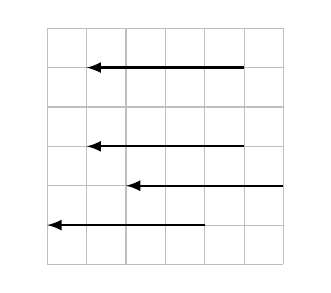
\begin{tikzpicture}[x=.5cm, y=.5cm,domain=-9:9,smooth, cross/.style={draw, cross out,
  minimum size=2*(#1-1pt), inner sep=0pt, outer sep=0pt},>=latex, font= \footnotesize]
   %Raster zeichnen
   \draw [color=gray!50]  [step=5mm] (-1,-1) grid (5,5);

\coordinate(a) at (4,4);
\coordinate(b) at (0,4);

\coordinate(c) at (4,2);
\coordinate(d) at (0,2);

\coordinate(e) at (5,1);
\coordinate(f) at (1,1);

\coordinate(g) at (3,0);
\coordinate(h) at (-1,0);
%Vektor
\draw[thick, ->] (a) node[right]{} -- (b) node[left]{};
\draw[thick, ->] (c) node[right]{} -- (d) node[left]{};
\draw[thick, ->] (e) node[right]{} -- (f) node[left]{};
\draw[thick, ->] (g) node[right]{} -- (h) node[left]{};
\end{tikzpicture}
\end{center}
Alle drei Pfeile sind Repräsentanten des selben Vektors.
\end{defi}
\begin{merke}{Bezeichnungen}{}\index{Vektoren!Bezeichnung}
Vektoren werden mit kleinen lateinischen Buchstaben und einem Pfeil gekennzeichnet $\vec{u}$. Verläuft ein Repräsentant eines Vektors von einem Punkt z.B. $P$ zu einem zweiten Punkt z.B. $Q$, so bezeichnet man alle Repräsentanten mit $\vv{PQ}$.
\begin{center}

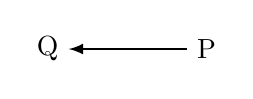
\begin{tikzpicture}[x=.5cm, y=.5cm,domain=-9:9,smooth, cross/.style={draw, cross out,
  minimum size=2*(#1-1pt), inner sep=0pt, outer sep=0pt},>=latex, ]
   %Raster zeichnen
% \draw [color=gray!50]  [step=5mm] (0,0) grid (3,3);
\coordinate(a) at (3,3);
\coordinate(b) at (0,3);
%Vektor
\draw[thick, ->] (a) node[right]{P} -- (b) node[left]{Q};
\end{tikzpicture}
\end{center}
\end{merke}
\begin{satz}{Vektoraddition}{}\phantomsection\label{vekadd}\index{Vektoren!Addition}
Bei der Addition von zwei Vektoren wird an den Endpunkt eines Repräsentanten des ersten Vektors $\vv{a}$ der Beginn eines Repräsentanten des zweiten Vektors $\vv{b}$ gesetzt. Der Pfeil des Summenvektors $\vv{c} = \vv{a} + \vv{b}$ ergibt sich durch den Pfeil der am Anfangspunkt des Vektors $\vv{a}$ beginnt und am Endpunkt des Vektors $\vv{b}$ endet.\\
Da es für einen Vektor unendlich viele Repräsentanten gibt, gibt es immer einen, der an der \glqq richtigen\grqq{} Stelle für eine Addition liegt.
\begin{center}
 
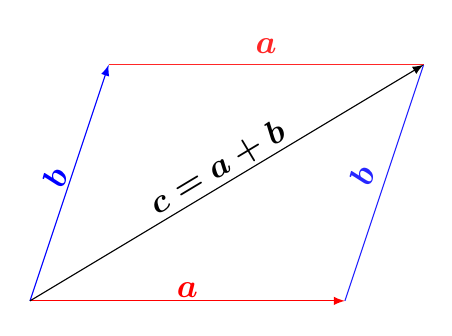
\begin{tikzpicture}[font=\boldmath]\large
    % Punkte
    \coordinate (A) at (0,0) {};
    \coordinate (B) at (4,0) {};
    \coordinate (C) at (1,3) {};
    \coordinate (D) at (5,3) {};

    % Draw the triangle
    \draw[blue!85]  (B) -- (D) node[sloped,midway,above] {$\vv{b}$};
    \draw[red!85]   (C) -- (D) node[sloped,midway,above] {$\vv{a}$};;
    \draw[->,  red,   arrows={-latex}]  (A) -- (B) node[sloped,midway,above=-0.1cm] {$\vv{a}$};
    \draw[->,  blue,  arrows={-latex}]  (A) -- (C) node[sloped,midway,above=-0.1cm] {$\vv{b}$};
    \draw[->, black, arrows={-latex}]  (A) -- (D) node[sloped,midway,above=-0.1cm] {$\vv{c} = \vv{a} + \vv{b} $};
\end{tikzpicture}
\end{center}
\end{satz}
\begin{satz}{Kommutativgesetz der Vektoraddition}{}\phantomsection\label{komuvekadd}
  Wie aus der Zeichnung bei Satz \ref{vekadd} leicht ersichtlich ist, ist die Addition von Vektoren kommutativ. Es gilt also: $$\vv{a} + \vv{b} = \vv{b} +\vv{a}$$ 
\end{satz}
\begin{satz}{Kommutativgesetz der Vektoraddition}{}
  Wie aus der Zeichnung bei Satz \ref{vekadd} leicht ersichtlich ist, ist die Addition von Vektoren kommutativ. Es gilt also: $$\vv{a} + \vv{b} = \vv{b} +\vv{a}$$ 
\end{satz}

\begin{satz}{Assoziativgesetz der Vektoraddition}{}\phantomsection\label{assivekadd}
\begin{center}
 Bei der Addition von Vektoren gilt das Assoziativgesetz. Es gilt also:
 $$(\vv{a} + \vv{b}) + \vv{c} = \vv{a} + (\vv{b} + \vv{c}) = \vv{a} + \vv{b} +\vv{c}$$
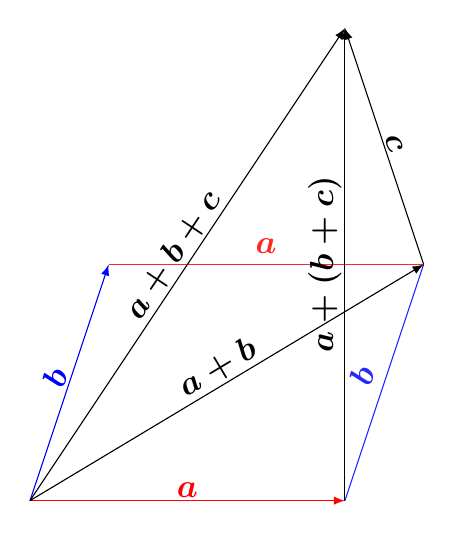
\begin{tikzpicture}[font=\boldmath]\large
    % Punkte
    \coordinate (A) at (0,0) {};
    \coordinate (B) at (4,0) {};
    \coordinate (C) at (1,3) {};
    \coordinate (D) at (5,3) {};
    \coordinate (E) at (4,6) {};

    % Draw the triangle
    \draw[blue!85]  (B) -- (D) node[sloped,midway,above] {$\vv{b}$};
    \draw[red!85]   (C) -- (D) node[sloped,midway,above] {$\vv{a}$};
    \draw[->,  red,   arrows={-latex}]  (A) -- (B) node[sloped,midway,above=-0.1cm] {$\vv{a}$};
    \draw[->,  blue,  arrows={-latex}]  (A) -- (C) node[sloped,midway,above=-0.1cm] {$\vv{b}$};
    \draw[->, black, arrows={-latex}]  (A) -- (D) node[sloped,midway,above=-0.1cm] {$ \vv{a} + \vv{b} $};
    \draw[->,  black,   arrows={-latex}]  (D) -- (E) node[sloped,midway,above=-0.1cm] {$\vv{c}$};
    \draw[->,  black,   arrows={-latex}]  (A) -- (E) node[sloped,midway,above=-0.1cm] {$\vv{a} + \vv{b} + \vv{c}$};
     \draw[->,  black,   arrows={-latex}]  (B) -- (E) node[sloped,midway,above=-0.1cm] {$\vv{a} + (\vv{b} + \vv{c})$};
\end{tikzpicture}
\end{center}
\end{satz}
\begin{b8d}{Besondere Vektoren}{}\index{Vektoren!Nullvektor}\index{Vektoren!Gegenvektor}
Bei der Rechnung mit Vektoren gibt es zwei besondere Vektoren zu betrachten. Hierbei handelt es sich um den sogenannten Nullvektor und den Gegenvektor.\\
Der Nullvektor $\vv{o}$ ist derjenige Vektor, der die Länge Null hat und bei dem sich bei er Addition mit anderen Vektoren nichts ändert. Es gilt: $$\vv{a} +\vv{o} = \vv{o} +\vv{a} = \vv{a}$$
Der Gegenvektor $-\vv{a}$ ist derjenige Vektor, der genauso lang wie der Vektor $\vv{a}$ ist allerdings entgegengerichtet. Für den Gegenvektor $-\vv{a}$ und den Vektor $\vv{a}$ gilt: $$\vv{a} +( -\vv{a} ) =\vv{a}-\vv{a}= \vv{o}$$
\end{b8d}
\begin{bem}{Vektorkette}{}\index{Vektoren!Vektorkette}
Werden mehrere Vektoren addiert so werden die jeweiligen Repräsentanten aneinandergereiht und das Ergebnis nennt man dann Vektorkette.
\end{bem}
\subsection{Vektor und Skalar}
\begin{merke}{Skalar}{}\index{Vektoren!Skalar}
   In der Analytischen Geometrie versteht man unter einem Skalar eine beliebige reelle Zahl. 
\end{merke}
\begin{defi}{Skalare Multiplikation}{}\index{Vektoren!Skalare Multiplikation}
Ein Vektor kann mit einer reellen Zahl durch eine Multiplikation verknüpft werden. Der Vektor $\lambda \cdot \vv{u}$ ist $|\lambda|$-mal so lang wie der Vektor $\vv{u}$. Dabei gilt für dis Zahl $\lambda$ folgendes $\lambda \in \mathds{R}$.\\
Für $\lambda > 0$ hat der Vektor $\lambda \cdot \vv{u}$ die gleiche Richtung wie der Vektor $\vv{u}$.\\
Für $\lambda < 0$ hat der Vektor $\lambda \cdot \vv{u}$ die entgegengesetzte Richtung wie der Vektor  $\vv{u}$.\\
\begin{center}
\begin{tikzpicture}[font=\boldmath]\large
    % Punkte
    \coordinate (A) at (0,0) {};
    \coordinate (B) at (2,1) {};
    \coordinate (C) at (6,2) {};
    \coordinate (D) at (2,0) {};
    \draw[->,  arrows={-latex}]  (A) -- (B) node[sloped,midway,above=-0.1cm] {$\vv{u}$};
    \draw[->,  arrows={-latex}]  (D) -- (C) node[sloped,midway,above=-0.1cm] {$2\cdot \vv{u}$};   
\end{tikzpicture}
\end{center}
\end{defi}
\begin{satz}{Rechenregeln für das Skalarprodukt}{}\index{Vektoren!Skalare Multiplikation}
Die Skalare Multiplikation folgt zwei Gesetzmäßigkeiten. dabei gilt $\lambda, \mu \in \mathds{R}$:
\begin{itemize}
    \item Assoziativgesetz: $\lambda \cdot \left(\mu \cdot \vv{u}\right) =\left( \mu \cdot \lambda \right)\vv{u}$
    \item Distributivgesetz 1: $\lambda \cdot \left(\vv{u} + \vv{v}\right) =\lambda \cdot \vv{u} + \lambda \cdot \vv{v} $
    \item Distributivgesetz 2: $\left( \lambda + \mu\right) \cdot \vv{u} =\lambda \cdot \vv{u} + \mu \cdot \vv{u}  $
\end{itemize}
\end{satz}
\begin{bem}{}{}
Beim aufstellen einer Vektorkette versucht man den Anfangs- und Endpunkt eines Vektors durch bekannte Vektoren zu verbinden. Der Vektor $\vv{AB}$ beginnt im Punkt $A$ und endet im Punkt $B$.

\end{bem}
\begin{bsp}{Vektorkette}{}
Die Vektoren $\vv{a}=\vv{AB}, \vv{b}=\vv{AD}$ und $\vv{c}=\vv{AS}$  spannen eine vierseitige Pyramide ABCDS auf, deren Grundfläche ein Parallelogramm ABCD ist. Der Fußpunkt der Pyramidenhöhe ist der Schnittpunkt der Diagonalen der Grundfläche.   
\begin{center}
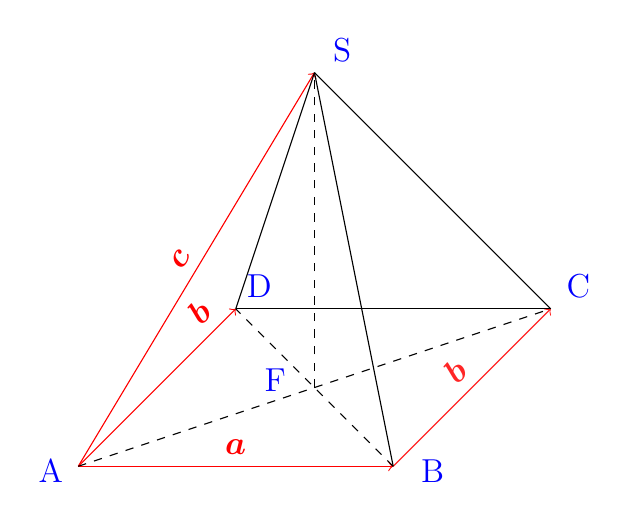
\begin{tikzpicture}[font=\boldmath]\large
    % Punkte
    \coordinate (A) at (0,0) {};
     \draw[blue] (-0.35,-0.35)   node [above] {A};
    \coordinate (B) at (4,0) {};
    \draw[blue] (4.5,-0.35)   node [above] {B};
    \coordinate (C) at (6,2) {};
    \draw[blue] (6.35,2)   node [above] {C};
    \coordinate (D) at (2,2) {};
    \draw[blue] (2.3,2)   node [above] {D};
    \coordinate (E) at (3,5) {};
    \draw[blue] (3.35,5)   node [above] {S};
    \coordinate (F) at (3,1) {};
    \draw[blue] (2.5,0.8)   node [above] {F};
    \draw[->, red]  (A) -- (B) node[sloped,midway,above] {$\vv{a}$};
    \draw[->,red!85]  (B) -- (C) node[sloped,midway,above] {$\vv{b}$};
    \draw  (C) -- (D) node[] {};
    \draw[->,red]  (A) -- (D) node[sloped,above,very near end] {$\vv{b}$};
   \draw[->,red]  (A) -- (E) node[sloped,midway,above] {$\vv{c}$};
   \draw  (E) -- (B) node[] {};
   \draw  (E) -- (C) node[] {};
   \draw  (E) -- (D) node[] {};
   \draw[dashed]  (A) -- (C) node[] {};
   \draw[dashed]  (B) -- (D) node[] {};
   \draw[dashed]  (F) -- (E) node[] {};

\end{tikzpicture}
\end{center}
Folgende Aufgaben sind typisch für Vektorketten
\begin{enumerate}
    \item Warum repräsentieren die Vektoren $\vv{BS}, \vv{CS}$ und $\vv{DS}$ \textcolor{red}{nicht} den Vektor $\vv{c}$?
    \begin{itemize}
        \item $\vv{BS}, \vv{CS}$ und $\vv{DS}$ sind gleich lang wie $\vv{c}$
        \item aber nicht \textcolor{red}{parallel} zu $\vv{c}$
    \end{itemize}
    \item Drücke die Vektoren $\vv{BS}, \vv{CS}, \vv{DS}$ und $\vv{AF}$ mithilfe der Vektoren $\vv{a}, \vv{b}$ und $\vv{
    c}$ aus.
    \begin{itemize}
        \item $\vv{BS}$
        \begin{itemize}
            \item[$\circ$] Um vom Startpunkt $B$ zum Endpunkt $S$ zu kommen, muss man von $B$ nach $A$ und dann nach $S$ \glqq laufen\grqq{}
            \item[$\circ$] $\vv{BS} = -\vv{a} + \vv{c} = \vv{c} - \vv{a}$
        \end{itemize}       
        \item $\vv{CS}$ 
        \begin{itemize}
            \item[$\circ$] Der Vektor $\vv{BC}$ ist ein Repräsentatnt des Vektors $\vv{b}$ 
            \item[$\circ$] $\vv{CS} = -\vv{b} - \vv{a} + \vv{c} = \vv{c} - \vv{a} -\vv{b}$
        \end{itemize}
        \item $\vv{DS}$ 
        \begin{itemize}
            \item[$\circ$] $\vv{DS} = -\vv{b} + \vv{c} = \vv{c} - \vv{b}$
        \end{itemize}
         \item $\vv{AF}$ 
         \begin{itemize}
             \item[$\circ$] Der Punkt $F$ liegt in der Mitte des Vektors $\vv{AC}$
             \item[$\circ$] $\vv{AC} = \vv{a} + \vv{b}$
             \item[$\circ$] $\vv{AF} = \dfrac{1}{2} \left(\vv{a} + \vv{b} \right)$
         \end{itemize}
    \end{itemize}
    \end{enumerate}
 In der Pyramide ist $M$ der Mittelpunkt der Seitenkante $\vv{BS}$ und $N$ der Mittelpunkt der Seitenkante  $\vv{CS}$.  
      \begin{enumerate}
        \item[3.] Drücke den Vektor $\vv{FN}$ mithilfe der Vektoren $\vv{a}, \vv{b}$ und $\vv{
    c}$ aus.
    \end{enumerate}
   \begin{multicols}{2}
    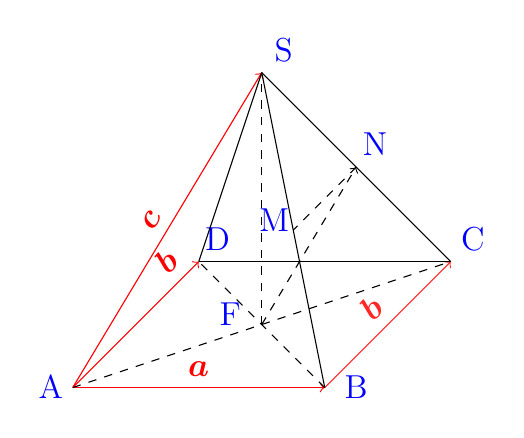
\begin{tikzpicture}[font=\boldmath, scale=0.8]\large
    % Punkte
    \coordinate (A) at (0,0) {};
     \draw[blue] (-0.35,-0.35)   node [above] {A};
    \coordinate (B) at (4,0) {};
    \draw[blue] (4.5,-0.35)   node [above] {B};
    \coordinate (C) at (6,2) {};
    \draw[blue] (6.35,2)   node [above] {C};
    \coordinate (D) at (2,2) {};
    \draw[blue] (2.3,2)   node [above] {D};
    \coordinate (E) at (3,5) {};
    \draw[blue] (3.35,5)   node [above] {S};
    \coordinate (F) at (3,1) {};
    \draw[blue] (2.5,0.8)   node [above] {F};
    \coordinate (G) at (4.5,3.5) {};
    \draw[blue] (4.8,3.5)   node [above] {N};
    \coordinate (H) at (3.5,2.5) {};
    \draw[blue] (3.2,2.3)   node [above] {M};
    \draw[->, red]  (A) -- (B) node[sloped,midway,above] {$\vv{a}$};
    \draw[->,red!85]  (B) -- (C) node[sloped,midway,above] {$\vv{b}$};
    \draw  (C) -- (D) node[] {};
    \draw[->,red]  (A) -- (D) node[sloped,above,very near end] {$\vv{b}$};
   \draw[->,red]  (A) -- (E) node[sloped,midway,above] {$\vv{c}$};
   \draw  (E) -- (B) node[] {};
   \draw  (E) -- (C) node[] {};
   \draw  (E) -- (D) node[] {};
   \draw[dashed]  (A) -- (C) node[] {};
   \draw[dashed]  (B) -- (D) node[] {};
   \draw[dashed]  (F) -- (E) node[] {};
    \draw[dashed]  (G) -- (H) node[] {};
    \draw[->,dashed]  (F) -- (G) node[] {};
\end{tikzpicture} 
    \begin{itemize}
        \item[$\circ$] Vektorkette von $F$ nach $C$ zu $N$.
     \begin{equation*}
            \begin{split}
                \vv{FN} &= \vv{FC} + \vv{CN}\\
                &=\vv{AF} + \dfrac{1}{2} \vv{CS}\\
                &= \dfrac{1}{2} \left(\vv{a} + \vv{b} \right) + \dfrac{1}{2}\left(\vv{c} - \vv{a} -\vv{b}\right)\\
                &=\dfrac{1}{2} \vv{a} + \dfrac{1}{2} \vv{b} + \dfrac{1}{2} \vv{c} - \dfrac{1}{2} \vv{a} -\dfrac{1}{2} \vv{b} \\
                &= \dfrac{1}{2}\vv{c}
            \end{split}
        \end{equation*}
        
    \end{itemize}
   \end{multicols}
   \begin{itemize}
       \item[$\circ$] Daraus folgt, dass der Vektor $\vv{FN}$ parallel und gleichgerichtet zum Vektor $\vv{c}$ aber nur halb so lang ist.
   \end{itemize}
   \begin{enumerate}
    \item[4.] Drücke den Vektor $\vv{MN}$ mithilfe der Vektoren $\vv{a}, \vv{b}$ und $\vv{
    c}$ aus.
    \begin{multicols}{2}
    \begin{itemize}
        \item[$\circ$] Vektorkette von $M$ über $B, C$ zum Punkt $N$.
     \begin{equation*}
            \begin{split}
                \vv{MN} &= - \dfrac{1}{2}\vv{BS} + \vv{BC} + \dfrac{1}{2} \vv{CS}\\
                &= -\dfrac{1}{2} \left( \vv{c} - \vv{a}\right) +\vv{b} + \dfrac{1}{2} \left(\vv{c} - \vv{a} -\vv{b}\right)\\
                &= -\dfrac{1}{2} \vv{c} +\dfrac{1}{2} \vv{a} +\vv{b} + \dfrac{1}{2} \vv{c} - \dfrac{1}{2}\vv{a} -\dfrac{1}{2}\vv{b}\\
                &= \dfrac{1}{2} \vv{b}
            \end{split}
        \end{equation*}  
        \item[$\circ$] Damit folgt, das die Mittellinie $\overline{MN}$ parallel, gleichgerichtet aber nur halb so lang wie der Vektor $\vv{b}$ ist.
    \end{itemize}
    \end{multicols}
\end{enumerate}
\end{bsp}
\section{Der Vektorraum}
\begin{defi}{Der Vektorraum}{}\index{Vektoren!Vektorraum}
    Die Menge aller Vektoren, in der die Gesetze der Addition von Vektoren und deren Multiplikation mit Skalaren gelten, nennt man Vektorraum. Die Basis des Vektorraums setzt sich aus der minimalen Anzahl von Vektoren zusammen die man braucht, um alle anderen Vektoren darstellen zu können. Die Anzahl dieser Vektoren bildet die Dimension des Vektorraums.
\end{defi}
\begin{merke}{Das orthonormale Koordinatensystem}{}\index{Vektoren!orthonormales Koordinatensystem}
    Das zweidimensionale und das dreidimensionale Koordinatensystem der Schulgeometrie ist ein orthonormales Koordinatensystem. Das bedeutet, die Basis besteht aus 2 bzw. 3 Vektoren der Länge eins welche paarweise senkrecht aufeinander stehen. Man bezeichnet diese Vektoren mit $\vv{e}_1, \vv{e}_2, \vv{e}_3$. 
\end{merke}
\begin{b8d}{Die Basisvektoren}{}\index{Vektoren!Basisvektoren}
Für die Basisvektoren $e_1, e_2$ und $e_3$ gilt folgende Darstellung:\\
$$\vv{e}_1 =\begin{pmatrix} 1 \\ 0 \\0 \end{pmatrix}, 
\vv{e}_2 =\begin{pmatrix} 0 \\ 1 \\0 \end{pmatrix}, 
\vv{e}_3 =\begin{pmatrix} 0 \\ 0 \\1 \end{pmatrix}$$
Mit den Basisvektoren ist man in der Lage, jeden Vektor durch eine Addition der Basisvektoren darzustellen. Diese Darstellung bezeichnet man als Spaltendarstellung der Vektoren. Der Vektor $\vv{a}$ hat damit die Darstellung $\vv{a} = \begin{pmatrix} a_1 \\ a_2 \\a_3 \end{pmatrix} = a_1\cdot \vv{e}_1 + a_2 \cdot \vv{e}_2 + a_3\cdot \vv{e}_3$ mit $a_1, a_2, a_3 \in \mathds{R}$. Die reellen Zahlen $a_i$ nennt man Koordinanten des Vektors $\vv{a}$.  
\end{b8d}
\begin{bem}{Rechnungen mit Vektoren}{}
\begin{itemize}
    \item Addition von Vektoren in der Spaltenschreibweise: Die Vektoren der $\vv{a}$ und $\vv{b}$ werden wie folgt addiert: $$\vv{a} + \vv{b} = \begin{pmatrix} a_1 \\ a_2 \\a_3 \end{pmatrix} + \begin{pmatrix} b_1 \\ b_2 \\b_3 \end{pmatrix} = \begin{pmatrix} a_1 + b_1 \\ a_2 + b_2 \\a_3 + b_3 \end{pmatrix}$$ dabei gilt $a_i, b_i \in \mathds{R}$.
    \item Multiplikation eines Vektors mit einem Skalar: Ein Vektor wird mit einem Skalar wie folgt multipliziert $$\lambda \cdot \vv{a} = \lambda \cdot \begin{pmatrix} a_1 \\ a_2 \\a_3 \end{pmatrix} = \begin{pmatrix} \lambda \cdot a_1 \\ \lambda \cdot a_2 \\\lambda \cdot a_3 \end{pmatrix}$$ mit $\lambda , a_i \in \mathds{R}$.
\end{itemize}
\end{bem}
\begin{satz}{Ortsvektoren}{}\index{Vektoren!Ortsvektor}
Jeder Punkt $P(p_1|p_2|p_3)$ mit $p_i \in \mathds{R}$ des dreidimensionalen Vektorraums lässt sich wie folgt in der Spaltenschreibweise schreiben:
$$\vv{P} = \begin{pmatrix} p_1 \\ p_2 \\p_3 \end{pmatrix}.$$ 
Dieser Vektor repräsentiert genau einen Pfeil der im Urpsrung des Koordinatensystems beginnt und an den Koordinaten des Punktes $P$ endet.\\ 
Diesen Pfeil nennt man Ortsvektor des Punktes $P$.
\end{satz}
\begin{satz}{Verbindungsvektoren}{}
Wird durch den Punkt $A(a_1|a_2|a_3)$ der Anfangspunkt und durch den Punkt $B(b_1|b_2|b_3)$ der Endpunkt eines Vektors festgelegt, so nennt man den dadurch entstehenden Vektor $\vv{AB}$ einen Verbindungsvektor. \\
Die Koordinaten des Verbindungsvektors berechnen sich wie folgt: $$\vv{AB} = \vv{B} -\vv{A} = \begin{pmatrix} b_1 \\ b_2 \\b_3 \end{pmatrix} - \begin{pmatrix} a_1 \\ a_2 \\a_3 \end{pmatrix} = \begin{pmatrix} b_1 - a_1 \\b_2 - a_2 \\b_3 -a_3 \end{pmatrix}$$
für alle $a_i, b_i \in \mathds{R}$.
\end{satz}
\begin{bsp*}{Orts- und Verbindungsvektor}{}

Gegeben sind die Punkte $P,R$ und $S$ im euklidischen Koordinatensystem. Die Punkte haben folgende Koordinaten: $P(2|3|2), R(3|3|0)$ und $S(0|4|2)$. Damit ergeben sich die die Ortsvektoren:
$$\vv{P} = \begin{pmatrix} 2 \\ 3 \\2 \end{pmatrix}, \vv{R} = \begin{pmatrix} 3 \\ 3 \\0 \end{pmatrix}, \vv{S}=\begin{pmatrix} 0 \\4 \\2 \end{pmatrix}.$$ Die Koordinaten des Verbindungsvektors berechnen sich damit wie folgt:
$$\vv{RS} = \vv{S} - \vv{R} = \begin{pmatrix} 0 \\4 \\2 \end{pmatrix} - \begin{pmatrix} 3 \\ 3 \\0 \end{pmatrix}=  \begin{pmatrix} -3 \\ 1 \\2 \end{pmatrix}$$
\tdplotsetmaincoords{70}{120}
\begin{tikzpicture}[scale=2, tdplot_main_coords, axis/.style={-> }, 
vector/.style={-stealth,red}, 
vector guide/.style={dashed,red}]
% -- remove these 3 lines if no axis is preferred
\draw[axis] (0, 0, 0) -- (5, 0, 0) node [left] {$x_1$};
\draw[axis] (0, 0, 0) -- (0, 5, 0) node [above] {$x_2$};
\draw[axis] (0, 0, 0) -- (0, 0, 2) node [above] {$x_3$};
% define points
\coordinate  (d1) at (0,0,0){};
\coordinate  (d2) at (4,0,0){};
\coordinate  (d3) at (2,3,2){};
\coordinate  (d4) at (0,4,2){};
\coordinate  (d5) at (3,3,0){};
\draw[blue] (2,3,2)   node [above] {$P$};
\draw[vector] (d1) -- (d3);
 %\draw (0,0,0) -- ++(-2.5pt,-2.5pt) -- ++(5pt,5pt) ++(-5pt,0pt) -- ++(5pt,-5pt);
  %\draw (2,3,2) -- ++(-2.5pt,-2.5pt) -- ++(5pt,5pt) ++(-5pt,0pt) -- ++(5pt,-5pt);
\draw[vector] (d5) -- (d4);
\draw[blue] (3,3,0)   node [above] {$R$};
\draw[blue] (0,4,2)   node [above] {$S$};
\draw[vector, blue, dashed] (d1) -- (d4);
\draw[vector, blue, dashed] (d1) -- (d5);
\draw[blue] (1.5,1.5,0)   node [above] {$\vv{R}$};
\draw[blue] (0,2,0.6)   node [above] {$\vv{S}$};
\draw[blue] (0,1,0.6)   node [above] {$\vv{P}$};
\end{tikzpicture}
\end{bsp*}
Durch die Verwendung von Koordinaten in der Vektorgeometrie ist es möglich spezielle Punkte relativ einfach zu berechnen. So ist es jetzt möglich, dass man zum Beispiel eine den Mittelpunkt einer Strecke bestimmt oder eine Strecke zu verdoppeln.
\begin{b8d*}{Eigenschaften einer Strecke}{}
Für den Ortsvektor $\vv{M}$ des Mittelpunktes der Strecke $\overline{AB}$ gilt: $$\vv{M} = \dfrac{1}{2}\left(\vv{A} + \vv{B}\right).$$
Die Strecke $\overline{AB}$ lässt sich so, einfach in beliebig viele Teile einteilen. 
\end{b8d*}
\begin{bsp*}{Teilungen einer Strecke}{}
Die Punkte $A$ und $B$ mit den Koordinaten $\vv{A} = \begin{pmatrix} 4 \\0 \\2 \end{pmatrix}$ und $\vv{B}= \begin{pmatrix} -2 \\3 \\5 \end{pmatrix}$ bestimmen eine Strecke $\overline{AB}$. Um die Strecke in vier gleich große Teile einzuteilen bestimmt man als erstes den Mittelpunkt. $$\vv{M_1}=\dfrac{1}{2}\left(\vv{A} + \vv{B}\right) = \dfrac{1}{2}\left( \begin{pmatrix} 4 \\0 \\2 \end{pmatrix} +  \begin{pmatrix} -2 \\3 \\5 \end{pmatrix} \right)= \dfrac{1}{2}\begin{pmatrix} 2 \\3 \\7 \end{pmatrix} = \begin{pmatrix} 1 \\1,5 \\3,5 \end{pmatrix}. $$ 
Anschließend werden die Mittelpunkte der Strecken $\overline{AM_1}$ und $\overline{M_1B}$ berechnet.
$$\vv{M_2} = \dfrac{1}{2}\left(\vv{A} + \vv{M_1}\right) =  \dfrac{1}{2} \left( \begin{pmatrix} 4 \\0 \\2 \end{pmatrix}  + \begin{pmatrix} 1 \\1,5 \\3,5 \end{pmatrix} \right) = \dfrac{1}{2} \begin{pmatrix} 5 \\1,5 \\5,5 \end{pmatrix} = \begin{pmatrix} 2,5 \\0,75 \\2,75 \end{pmatrix}$$
$$\vv{M_3} = \dfrac{1}{2}\left(\vv{M_1} + \vv{B}\right) =  \dfrac{1}{2} \left( \begin{pmatrix} 1 \\1,5 \\3,5 \end{pmatrix} +   \begin{pmatrix} -2 \\3 \\5 \end{pmatrix} \right) = \dfrac{1}{2} \begin{pmatrix} -1 \\4,5 \\8,5 \end{pmatrix} =  \begin{pmatrix} -0,5 \\2,25 \\4,25 \end{pmatrix}$$
Durch die Berechnung der Punkte ergeben sich 4 gleich große Teilstücke. \\
Die Strecken $\overline{AM_2}, \ \overline{M_2M_1}, \ \overline{M_1M_3}$ und $\overline{M_3B}.$
\begin{center}
 
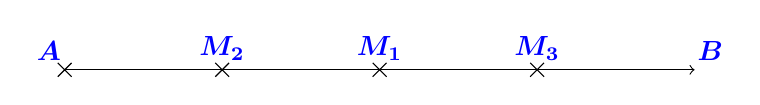
\begin{tikzpicture}[font=\boldmath]
    % Punkte
    \coordinate (C) at (1,3) {};
    \coordinate (D) at (9,3) {};   
    
    \draw[->]  (C) -- (D) node[sloped,midway,above] {};
    \draw[blue] (0.8,3)   node [above] {$A$};
    \draw (1, 3) -- ++(-2.5pt,-2.5pt) -- ++(5pt,5pt) ++(-5pt,0pt) -- ++(5pt,-5pt);
    \draw[blue] (9.2,3)   node [above] {$B$};
       % \draw (9, 3) -- ++(-2.5pt,-2.5pt) -- ++(5pt,5pt) ++(-5pt,0pt) -- ++(5pt,-5pt);
 \draw[blue] (5,3)   node [above] {$M_1$};
        \draw (5, 3) -- ++(-2.5pt,-2.5pt) -- ++(5pt,5pt) ++(-5pt,0pt) -- ++(5pt,-5pt);
 \draw[blue] (3,3)   node [above] {$M_2$};
        \draw (3, 3) -- ++(-2.5pt,-2.5pt) -- ++(5pt,5pt) ++(-5pt,0pt) -- ++(5pt,-5pt);
 \draw[blue] (7,3)   node [above] {$M_3$};
        \draw (7, 3) -- ++(-2.5pt,-2.5pt) -- ++(5pt,5pt) ++(-5pt,0pt) -- ++(5pt,-5pt);     
\end{tikzpicture} 
\end{center}
\end{bsp*}
Die Eigenschaften der Berechnung der Mittelpunkte lassen sich auch auf Flächen und Körper anwenden. So ist es jetzt möglich, den Schwerpunkt eines Dreiecks bzw. den Schwerpunkt einer dreiseitigen Pyramide zu bestimmen.
\begin{merke}{Schwerpunkte bei Strecke, Dreieck und Pyramide}{}\index{Schwerpunkt!Strecke}\index{Schwerpunkt!Dreieck}
\index{Schwerpunkt!Pyramide}

Mithilfe dieser Übersicht ist es möglich, die Ortskoordinaten des Schwerpunkts zu berechnen.\\[0.5cm]
\begin{center}
\bgroup
\def\arraystretch{1.5}%  1 is the default, change whatever you need
\begin{tabular}{|l|c|c|}
    \hline
    & Berechnung & Teilverhältnis \\[0.2cm]
     \hline
     \hline
     Schwerpunkt einer Strecke & $\vv{S_{AB}} = \dfrac{1}{2}(\vv{A} + \vv{B})$ & 1:1\\[0.2cm]
     \hline
     Schwerpunkt eines Dreiecks &$ \vv{S_{ABC}} = \dfrac{1}{3} (\vv{A} + \vv{B} + \vv{C})$ & 1:2\\[0.2cm]
     \hline
     Schwerpunkt einer Pyramide & $\vv{S_{ABCD}} = \dfrac{1}{4}(\vv{A} + \vv{B} +\vv{C} + \vv{D})$ & 1:3\\[0.2cm]
     \hline
\end{tabular}
\egroup
\end{center}
Das Teilverhältnis gibt an, in welchem Verhältnis der Schwerpunkt die einzelnen Teilstrecke unterteilt. So entstehen, zum Beispiel bei der Teilung einer Strecke, zwei gleich lange Teilstrecken.
\end{merke}
\section{Skalar- und Vektorprodukt}
\subsection{Das Skalarprodukt}
Um die Abstände im Raum berechnen zu können wird die Länge eines Vektors definiert.
\begin{defi}{Der Betrag eines Vektors}{}
Gegeben ist der Vektor $\vv{a}$ durch die Koordinaten $\vv{a} = \begin{pmatrix} a_1 \\a_2 \\a_3\end{pmatrix}$. Der Betrag des Vektors entspricht der Länge eines Repräsentanten des Vektors. Hierbei berechnet sich die Länge wie folgt: $$|\vv{a}| = \sqrt{a_1^2 + a_2^2 + a_3^2}$$
\end{defi}
Mit dem Betrag eines Vektors kann jetzt der Abstand zweier Punkte berechnet werden.
\begin{merke}{Abstand zweier Punkte}{}\index{Abstand zweier Punkte}
Durch die Berechnung des Betrags ist es möglich die Entfernung zweier Punkte im Raum zu berechnen. Dadurch haben die Punkte $A(a_1|a_2|a_3)$ und $B(b_1|b_2|b_3)$ die Entfernung: $$|\vv{AB}|=|\vec{B} - \vv{A}| = | \begin{pmatrix} b_1 \\b_2 \\b_3\end{pmatrix} -\begin{pmatrix} a_1 \\a_2 \\a_3\end{pmatrix}| = |\begin{pmatrix} b_1 - a_1 \\b_2 - a_2 \\b_3- a_3\end{pmatrix}| =\sqrt{(b_1-a_1)^2+ (b_2-a_2)^2 + (b_3-a_3)^2}$$
\end{merke}
\begin{bsp}{Berechnung von Längen}{}
Gegeben sind die Punkte $A(2|3|-1)$ und $B(-2|2|1)$. Der Orstvektor des Punktes $A$ hat damit die Länge $$|\vv{A}| = \sqrt{2^2 +3^2 +(-1)^2} = \sqrt{14}\ [LE]$$ und die Punkte $A$ und $B$ haben damit den Abstand $$|\vv{AB}| = |\begin{pmatrix} -2 \\2 \\1\end{pmatrix} - \begin{pmatrix} 2 \\3 \\-1\end{pmatrix}| = |\begin{pmatrix} -4 \\-1 \\2\end{pmatrix}| = \sqrt{(-4)^2 +(-1)^2 + (2)^2} = \sqrt{21} \ [LE]$$
\end{bsp}
Durch die Einführung des Abstands zweier Punkte ist man jetzt in der Lage neues Strukturen im Raum zu definieren. 
\begin{b8d}{Kugelgleichung}{}\index{Kugelgleichung}
Alle Punkte, die von einem gegeben Punkt $M(m_1|m_2|m_3)$ die gleiche Entfernung $r$ haben, liegen auf einer Kugel um den Mittelpunkt $r$. Die Koordinaten aller dieser Punkte $X(x_1|x_2|x_3)$ genügen folgender Gleichung: $$(x_1-m_1)^2 + (x_2 -m_2)^2 + (x_3 -m_3 ^2) = r^2$$
\end{b8d}
In der analytischen Geometrie ist es oft wichtig zu wissen, ob zwei Vektoren senkrecht aufeinander stehen. Diese Information ist mit Hilfe des Skalarprodukts bestimmbar.
\begin{merke}{Das Skalarprodukt}{}\index{Vektoren!Skalarprodukt}
Die Zahl $$\vv{a} \circ \vv{b} = \begin{pmatrix} a_1 \\a_2 \\a_3\end{pmatrix} \circ \begin{pmatrix} b_1 \\b_2 \\b_3\end{pmatrix} = a_1\cdot b_1 + a_2\cdot b_2 + a_3\cdot b_3$$ heißt Skalarprodukt der Vektoren $\vv{a}$ und $\vv{b}$. 
\end{merke}
Damit zwei Vektoren orthogonal bzw. senkrecht zueinander sind, muss für zwei Vektoren $\vv{a}$ und $\vv{b}$ folgende Gleichung gelten: $|\vv{a}|^2 + |\vv{b}|^2 = |\vv{b} -\vv{a}|^2$. Durch eine einfache Umformung der Gleichung folgt\\ $ a_1\cdot b_1 + a_2\cdot b_2 + a_3\cdot b_3 = 0$ und damit ergibt sich folgendes Kriterium.
\begin{b8d}{Orthogonalität von zwei Vektoren}{} \index{Vektoren!Orthogonalität}
Zwei vom Nullvektor verschiedene Vektoren $\vv{a}$ und $\vv{b}$ sind genau dann orthogonal zueinander, wenn ihr Skalarprodukt den Wert Null hat.
\end{b8d}
Schließen zwei Vektoren $\vv{a}$ und $\vv{b}$ einen von $90^{\circ}$ verschiedenen Winkel $\varphi$ ein, so lässt sich dieser wie folgt berechnen.
\begin{merke}{Winkel zwischen zwei Vektoren}{}
Der Winkel $\varphi$ zwischen zwei vom Nullvektor verschiedenen Vektoren $\vv{a}$ und $\vv{b}$ ergibt sich aus folgendem Zusammenhang: $$\cos{\varphi} = \dfrac{\vv{a} \circ \vv{b}}{|\vv{a}| \cdot |\vv{b}|}\hspace{0.5cm}\text{mit}\hspace{0.25cm} 0^{\circ} \leq \varphi \leq 180^{\circ}.$$ 
Die Größe des Winkels $\varphi$ bestimmt sich damit durch die Gleichung:
$$\varphi = \arccos{(\dfrac{\vv{a} \circ \vv{b}}{|\vv{a}| \cdot |\vv{b}|})} = \cos^{-1}{(\dfrac{\vv{a} \circ \vv{b}}{|\vv{a}| \cdot |\vv{b}|})}$$
\end{merke}
\begin{bsp}{Berechnung des Winkels zwischen zwei Vektoren}{}
Gegeben sind die Punkte $A(7|-3|4), B(2|2|4)$ und $C(2|-3|-1)$ die ein Dreieck festlegen. Berechne die Größe des Winkels $\alpha$.
\begin{center}
\begin{tikzpicture}
  \draw
    (3,-1) coordinate (a) node[right] {B}
    -- (0,0) coordinate (b) node[left] {A}
    -- (2,2) coordinate (c) node[above right] {C}
    -- (3,-1) 
    pic[draw=red, ->,  angle radius=1cm]
    {angle=a--b--c};
    \draw
    (0.4,0.2) coordinate (wink) node[right] {$\alpha$};
\end{tikzpicture}
\end{center}
Vorgehen zum berechnen des Winkels $\alpha$:
\begin{enumerate}
    \item Bestimmung der Vektoren $\vv{a} = \vv{AB}$ und $\vv{b} = \vv{AC}$.
    \begin{equation*}
        \begin{split}
            \vv{a} &= \vv{B} - \vv{A} = \begin{pmatrix} 2 \\2 \\4\end{pmatrix} -\begin{pmatrix} 7 \\-3 \\4\end{pmatrix} = \begin{pmatrix} -5 \\5\\0\end{pmatrix} 
            \end{split}
            \end{equation*}
    \begin{equation*}
        \begin{split}
            \vv{b} &= \vv{C} - \vv{A} = \begin{pmatrix} 2 \\-3 \\-1\end{pmatrix} -\begin{pmatrix} 7 \\-3 \\4\end{pmatrix} = \begin{pmatrix} -5 \\0\\-5\end{pmatrix} 
            \end{split}
            \end{equation*}
                
    \item Berechnung des Skalarprodukts.
    \begin{equation*}
        \begin{split}
            \vv{a} \circ \vv{b} &= \begin{pmatrix} -5 \\5 \\0\end{pmatrix} \circ \begin{pmatrix} -5 \\0 \\-5 \end{pmatrix} = 25 +0 +0 = 25
            \end{split}
            \end{equation*}
    \item Berechnung der Beträge der Vektoren $\vv{a}$ und $\vv{b}$.
    \begin{equation*}
        \begin{split}
            |\vv{a}| & = |\begin{pmatrix} -5 \\0\\-5\end{pmatrix}| =  \sqrt{(-5)^2 + (5)^2 + 0^2}  = \sqrt{25+25} = \sqrt{50} = 5\cdot \sqrt{2}\\
            |\vv{b}| &= |\begin{pmatrix} -5 \\0\\-5\end{pmatrix} |= \sqrt{(-5)^2 + 0^2 + (-5)^2} = \sqrt{25+25}= \sqrt{50} = 5\cdot \sqrt{2}
            \end{split}
            \end{equation*}
    \item Bildung des Quotienten und Berechnung des Winkels.
    \begin{equation*}
        \begin{split}
            \cos{(\alpha)} &= \dfrac{\vv{a}\circ \vv{b}}{|\vv{a}| \cdot |\vv{b}|}= \dfrac{25}{5\sqrt{2} \cdot 5\sqrt{2}}\\
            &= \dfrac{25}{50} = \dfrac{1}{2}\\
            \alpha &= \arccos{(\dfrac{1}{2})} = 60^{\circ}
            \end{split}
            \end{equation*}
\end{enumerate}
\end{bsp}
\subsection{Das Vektorprodukt}
\index{Vektoren!Vektorprodukt}
Das Vektorprodukt ist anders als das Skalarprodukt ein Vektor und keine Zahl. Gekennzeichnet wird das Vektorprodukt durch $\times$ statt durch das Multiplikationszeichen $\cdot$. \\
\begin{b8d*}{Vektorprodukt und Skalarprodukt}{}
Dadurch ergibt sich folgende Regel:\\
Bei der Schreibweise $\vv{a} \times\vv{b}$ ergibt sich ein Vektor $\vv{c}$,\\
bei der Schreibweise $\vv{a} \cdot \vv{b}$ ergibt sich eine Zahl $c\in \mathds{R}$.
\end{b8d*}
Das Vektorprodukt $\vv{a} \times \vv{b}$ aus den beiden Vektoren $\vv{a}$ und $\vv{b}$ ist ein Vektor, der die folgenden Eigenschaften besitzt.
\begin{merke}{Eigenschaften des Vektorprodukts}{}
   \begin{enumerate}
       \item $\vv{a} \times \vv{b} = 0$, falls der Vektor $\vv{a}$ bzw. der Vektor $\vv{b}$ der Nullvektor ist.
       \item $\vv{a} \times \vv{b} = 0$, falls der Vektor $\vv{a}$ und der Vektor $\vv{b}$ parallel zueinander sind.
       \item Der Betrag des Vektorprodukts gibt den Flächeninhalt des durch die Vektoren $\vv{a} $ und $\vv{b}$ aufgespannten Parallelogramms wieder. Es gilt damit $$F_P=|\vv{a} \times \vv{b} |.$$
       \item Der Flächeninhalt des durch drei Punkte aufgestellten Dreiecks berechnet sich durch den halben Betrag des Vektorprodukts: $$F_{\text{Dreieck}} = \dfrac{1}{2} |\vv{a} \times \vv{b}|$$
       \item Der resultierende Vektor $\vv{c} $ steht senkrecht sowohl auf dem Vektoren $\vv{a} $ als auch auf dem Vektor $\vv{b}$.
   \end{enumerate} 
\end{merke}
\begin{defi*}{Berechnung des Vektorprodukts}{}
Aus zwei Vektoren $\vv{a}\neq 0$ und $\vv{b} \neq 0$ ergibt sich der Vektor durch das Vektorprodukt wie folgt: $$\vv{a} \times \vv{b} = \begin{pmatrix} a_1 \\a_2\\a_3\end{pmatrix} \times \begin{pmatrix} b_1 \\b_2\\b_3\end{pmatrix} = \begin{pmatrix} a_2\cdot b_3 - a_3\cdot b_2 \\a_3\cdot b_1 - a_1\cdot b_3\\a_1\cdot b_2 - a_2\cdot b_1\end{pmatrix}$$
\end{defi*}
\begin{b8d*}{Berechnung des Vektorprodukts}{}
    Bei der Berechnung des Vektorprodukts ist es möglich die obige Variante benutzen oder eine vereinfachte Variante buntzen. Bei dieser Verkürzten Variante werden unter jeden Vektor jeweils die $x_1$ und $x_2$ Koordinaten des Vektors nochmals notiert und die erste Zeile der Vektoren durchgestrichen. Anschließend werden dann die Koordinaten über kreuz multipliziert und dann entsprechende subtrahiert.
\[
\begin{array}[t]{@{}c@{}}
\vv{c}=\begin{pmatrix} a_1 \\ a_2 \\ a_3 \end{pmatrix} \\ a_1 \\ a_2
\end{array}
\times
\begin{array}[t]{@{}c@{}}
\begin{pmatrix} b_1 \\ b_2 \\ b_3 \end{pmatrix} \\ b_1 \\ b_2
\end{array}
=
\begin{pmatrix}
a_2\cdot b_3-a_3\cdot b_2 \\
a_3\cdot b_1-a_1\cdot b_3 \\
a_1\cdot b_2-a_2\cdot b_1
\end{pmatrix}
\] 
\begin{center}
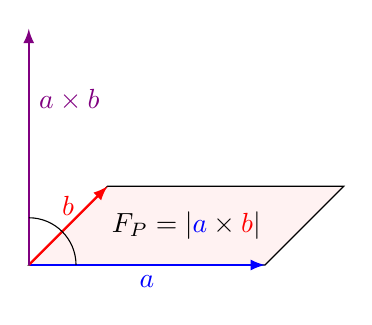
\begin{tikzpicture}
\draw[-,fill=white!95!red](0,0)--(3,0)--(4,1)--(1,1)--cycle;
\node at (2,0.5) {$F_P = |\textcolor{blue}{a}\times \textcolor{red}{b}|$};
\draw[thick,-latex,blue](0,0)--(3,0)node[midway,below]{$a$};
\draw[thick,-latex,red](0,0)--(1,1)node[midway,above]{$b$};
\draw[thick,-latex,blue!50!red](0,0)--(0,3)node[pos=0.7,right]{$a\times b$};
%\draw (0.6,0) arc [start angle=0,end angle=45,radius=0.6]
%node[pos=0.7,right]{$\varphi$};
\draw (0.6,0) arc [start angle=0,end angle=90,radius=0.6]
node[pos=0.7,right]{};
\end{tikzpicture}
\end{center}
\end{b8d*}
\begin{bsp}{Berechnung des Vektorprodukts}{}
Gegeben sind die Punkte $A(3|3|3), B(4|5|6)$ und $C(7|8|9)$. Durch die Bestimmung des Betrags des Vektorprodukts soll der Flächeninhalt des aufgespannten Dreiecks bestimmt werden.
\begin{equation*}
    \begin{split}
        F_{\text{Dreieck}} &= \dfrac{1}{2} \cdot |\vv{AB} \times \vv{AC}|\\
        &= \dfrac{1}{2} \cdot |\begin{pmatrix} 1 \\ 2 \\ 3 \end{pmatrix} \times \begin{pmatrix} 4 \\ 5 \\ 6 \end{pmatrix}|
        = \dfrac{1}{2} \cdot |
\begin{array}[t]{@{}c@{}}
\begin{pmatrix} \bcancel{1} \\ 2 \\ 3 \end{pmatrix} \\ 1 \\ 2
\end{array}
\times
\begin{array}[t]{@{}c@{}}
\begin{pmatrix} \bcancel{4} \\ 5\\ 6 \end{pmatrix} \\ 4 \\ 5
\end{array}|\\
&=
\dfrac{1}{2} \cdot |\begin{pmatrix}
2\cdot 6-3\cdot 5 \\
3\cdot 4-1\cdot 6 \\
1\cdot 5-2\cdot 4
\end{pmatrix}|
=\dfrac{1}{2} \cdot | \begin{pmatrix}
12-15 \\
12-6 \\
5-8
\end{pmatrix}| =\dfrac{1}{2} \cdot |\begin{pmatrix}
-3 \\
6 \\
-3
\end{pmatrix}|\\
&= \dfrac{1}{2} \cdot \sqrt{9+36+9} = \dfrac{1}{2} \cdot \sqrt{54} =\dfrac{3}{2} \cdot \sqrt{6} \ \text{[FE]} 
    \end{split}
\end{equation*}
\end{bsp}
\subsection{Das Spatprodukt}
\index{Vektoren!Spatprodukt}
Ein Spat ist ein geometrischer Körper, der sechs Parallelogramme als Seitenflächen besitzt. Die gegenüberliegende Parallelogramme sind immer kongruent zueinander und liegen in parallelen Ebenen.\\
Unter dem Spatprodukt versteht man das Skalarprodukt eines Vektors mit dem Vektorprodukt zweier weiterer Vektoren.
\begin{defi}{Das Spatprodukt}{}
Spannen die Vektoren $\vv{a}, \vv{b}$ und $\vv{c}$ einen Spat bzw. eine dreiseitige Pyramide auf, ist das Volumen:
$$V_{\text{Spat}} = |(\vv{a}\times\vv{b})\circ \vv{c}|$$ $$V_{\text{Pyramide}}=\dfrac{1}{6}|(\vv{a}\times\vv{b})\circ \vv{c}| $$
\end{defi} 
\begin{bsp}{Berechnung des Volumens einer dreiseitigen Pyramide I}{}
Durch die Vektoren $\vv{a} = \begin{pmatrix} 1\\2\\3
\end{pmatrix}, \vv{b}= \begin{pmatrix}
    2\\3\\1
\end{pmatrix}$ und $\vv{c}= \begin{pmatrix}
   3\\1\\2
\end{pmatrix}$ spannen eine dreiseitige Pyramide auf. Das Volumen dieser Pyramide bestimmt sich damit durch das Spatprodukt wie folgt:
\begin{equation*}
    \begin{split}
      V_{\text{Pyramide}} &= \dfrac{1}{6} \cdot |(\vv{a}\times \vv{b})\circ \vv{c}| = \dfrac{1}{6} \cdot |(\begin{pmatrix}1\\2\\3\end{pmatrix} \times 
\begin{pmatrix} 2\\3\\1 \end{pmatrix}) \circ 
\begin{pmatrix} 3\\1\\2 \end{pmatrix}|\\
&=\dfrac{1}{6} \cdot |\begin{pmatrix} -7\\5\\-1 \end{pmatrix}\circ \begin{pmatrix} 3\\1\\2 \end{pmatrix}|  =\dfrac{1}{6} \cdot |-18| = 3\ \text{[VE]}
    \end{split}
\end{equation*}
\end{bsp}

\begin{b8d*}{Berechnung der Determinante}{}
\index{Vektoren!Determinante}
    Das Spatprodukt lässt sich alternativ durch die Berechnung der sogenannten Determinante bestimmen. Die Determinante bestimmt sich durch das notieren der drei erzeugenden Vektoren in folgendes Schema:
\[
\det(\vv{a}, \vv{b}, \vv{c})
%
=\begin{matrix}\begin{tikzpicture}
\matrix [
matrix of math nodes,
column sep=1em,
row sep=1em,
] (sarrus) {
a_1 & b_1 & c_1  \\ a_2 & b_2 & c_2 \\ a_3 & b_3 & c_3 \\
};
% Striche
\path ($(sarrus-1-1.north west)-(0.5em,0)$) edge[] ($(sarrus-3-3.south east -| sarrus-1-1.north west)-(0.5em,0)$);
\path ($(sarrus-1-3.north east)+(0.5em,0)$) edge[] ($(sarrus-3-3.south east -| sarrus-1-3.north east)+(0.5em,0)$);
\end{tikzpicture}\end{matrix}
%
=\begin{matrix}\begin{tikzpicture}
\matrix [
matrix of math nodes,
column sep=1em,
row sep=1em,
%left delimiter={|} %,right delimiter={|}, 
] (sarrus) {
a_1 & b_1 & c_1 & a_1 & b_1 \\ a_2 & b_2 & c_2 & a_2 & b_2\\ a_3 & b_3 & c_3 & a_3 & b_3\\
};
% Striche
\path ($(sarrus-1-1.north west)-(0.5em,0)$) edge[] ($(sarrus-3-3.south east -| sarrus-1-1.north west)-(0.5em,0)$);
\path ($(sarrus-1-3.north east)+(0.5em,0)$) edge[] ($(sarrus-3-3.south east -| sarrus-1-3.north east)+(0.5em,0)$);
\path[->,blue] (sarrus-1-1) edge (sarrus-2-2)
(sarrus-2-2) edge (sarrus-3-3)
(sarrus-1-2) edge (sarrus-2-3)
(sarrus-2-3) edge (sarrus-3-4)
(sarrus-1-3) edge (sarrus-2-4)
(sarrus-2-4) edge (sarrus-3-5);
\path[->,red](sarrus-3-1) edge[dashed] (sarrus-2-2)
(sarrus-2-2) edge[dashed] (sarrus-1-3)
(sarrus-3-2) edge[dashed] (sarrus-2-3)
(sarrus-2-3) edge[dashed] (sarrus-1-4)
(sarrus-3-3) edge[dashed] (sarrus-2-4)
(sarrus-2-4) edge[dashed] (sarrus-1-5);

\foreach \c in{3,4,5} \node[blue] at (sarrus-3-\c.south east) {$+$};
\foreach \c in{3,4,5} \node[red] at (sarrus-1-\c.north east) {$-$};

% Strich rechts
\path ($(sarrus-1-5.north east)+(0.5em,0)$) edge[densely dotted] ($(sarrus-3-5.south east -| sarrus-1-5.north east)+(0.5em,0)$);
\end{tikzpicture}\end{matrix} 
\]
Aus der Determinante folgt damit für das Volumen folgende Rechnung:
\begin{equation*}
    \begin{split}
        V_{\text{Spat}} &= |\det(\vv{a}, \vv{b}, \vv{c})| \\
        &= |a_1\cdot b_2 \cdot c_3 + b_1\cdot c_2 \cdot a_3 + c_1\cdot a_2 \cdot b_3 - a_3\cdot b_2 \cdot c_1 - b_3\cdot c_2 \cdot a_1 - c_3\cdot a_2\cdot b_1|\\
        V_{\text{Pyramide}} &= \dfrac{1}{6}\cdot |\det(\vv{a}, \vv{b}, \vv{c})| \\ 
        &= \dfrac{1}{6}\cdot |a_1\cdot b_2 \cdot c_3 + b_1\cdot c_2 \cdot a_3 + c_1\cdot a_2 \cdot b_3 - a_3\cdot b_2 \cdot c_1 - b_3\cdot c_2 \cdot a_1 - c_3\cdot a_2\cdot b_1|
    \end{split}
\end{equation*}
\end{b8d*}
\begin{bsp}{Berechnung des Volumens einer dreiseitigen Pyramide II}{}
 Durch die Vektoren $\vv{a} = \begin{pmatrix} 1\\2\\3
\end{pmatrix}, \vv{b}= \begin{pmatrix}
    2\\3\\1
\end{pmatrix}$ und $\vv{c}= \begin{pmatrix}
   3\\1\\2
\end{pmatrix}$ spannen eine dreiseitige Pyramide auf. 
\[
\det(\vv{a}, \vv{b}, \vv{c})
%
=\begin{matrix}\begin{tikzpicture}
\matrix [
matrix of math nodes,
column sep=1em,
row sep=1em,
] (sarrus) {
1 & 2 & 3  \\ 2 &3 & 1 \\ 3 & 1 & 2 \\
};
% Striche
\path ($(sarrus-1-1.north west)-(0.5em,0)$) edge[] ($(sarrus-3-3.south east -| sarrus-1-1.north west)-(0.5em,0)$);
\path ($(sarrus-1-3.north east)+(0.5em,0)$) edge[] ($(sarrus-3-3.south east -| sarrus-1-3.north east)+(0.5em,0)$);
\end{tikzpicture}\end{matrix}
%
=\begin{matrix}\begin{tikzpicture}
\matrix [
matrix of math nodes,
column sep=1em,
row sep=1em,
%left delimiter={|} %,right delimiter={|}, 
] (sarrus) {
1 & 2 & 3 & 1 & 2 \\ 2 & 3 & 1 & 2 & 3\\ 3 & 1 & 2 & 3 & 1\\
};
% Striche
\path ($(sarrus-1-1.north west)-(0.5em,0)$) edge[] ($(sarrus-3-3.south east -| sarrus-1-1.north west)-(0.5em,0)$);
\path ($(sarrus-1-3.north east)+(0.5em,0)$) edge[] ($(sarrus-3-3.south east -| sarrus-1-3.north east)+(0.5em,0)$);
\path[->,blue] (sarrus-1-1) edge (sarrus-2-2)
(sarrus-2-2) edge (sarrus-3-3)
(sarrus-1-2) edge (sarrus-2-3)
(sarrus-2-3) edge (sarrus-3-4)
(sarrus-1-3) edge (sarrus-2-4)
(sarrus-2-4) edge (sarrus-3-5);
\path[->,red](sarrus-3-1) edge[dashed] (sarrus-2-2)
(sarrus-2-2) edge[dashed] (sarrus-1-3)
(sarrus-3-2) edge[dashed] (sarrus-2-3)
(sarrus-2-3) edge[dashed] (sarrus-1-4)
(sarrus-3-3) edge[dashed] (sarrus-2-4)
(sarrus-2-4) edge[dashed] (sarrus-1-5);

\foreach \c in{3,4,5} \node[blue] at (sarrus-3-\c.south east) {$+$};
\foreach \c in{3,4,5} \node[red] at (sarrus-1-\c.north east) {$-$};

% Strich rechts
\path ($(sarrus-1-5.north east)+(0.5em,0)$) edge[densely dotted] ($(sarrus-3-5.south east -| sarrus-1-5.north east)+(0.5em,0)$);
\end{tikzpicture}\end{matrix} 
\]
Aus der Determinante folgt damit für das Volumen folgende Rechnung:
\begin{equation*}
    \begin{split}
        V_{\text{Pyramide}} &= \dfrac{1}{6}\cdot |\det(\vv{a}, \vv{b}, \vv{c})| \\ 
        &= \dfrac{1}{6}\cdot |1\cdot 3 \cdot 2 + 2\cdot 1 \cdot 3 + 3\cdot 2 \cdot 1 - 3\cdot 3 \cdot 3 - 1\cdot 1 \cdot 1 - 2\cdot 2\cdot 2|\\
        &= \dfrac{1}{6} \cdot |6+6+6-27-1-8|\\
        &= \dfrac{1}{6} \cdot |-18| = 3 \ \text{[VE]}
    \end{split}
\end{equation*}
\end{bsp}
\section{Lineare Abhängigkeit und Unabhängigkeit}\index{Vektoren!Lineare Abhängigkeit}\index{Vektoren!Lineare Unabhängigkeit}
\begin{b8d}{Linearkombination}{}\index{Vektoren!Linearkombination}
Einen Term \(r\cdot \vv{a} + s\cdot \vv{b} + t \cdot \vv{c}\) mit \(r,s,t \in \mathds{R}\) bezeichnet man als Linearkombination der Vektoren \(\vv{a}, \vv{b}\) und \(\vv{c}\)
\end{b8d}
\begin{defi}{Lineare Abhängigkeit}{}
   Die Vektoren \(\vv{a_1}, \vv{a_2}, \ldots , \vv{a_n}\) heißen \textcolor{red}{\textbf{linear abhängig}}, wenn mindestens einer dieser Vektoren als Linearkombination der anderen Vektoren darstellbar ist.\\
   Andernfalls nennt man die Vektoren \textcolor{red}{\textbf{linear unabhängig}}, d.h.: Die Vektoren 
   \(\vv{a_1}, \vv{a_2}, \ldots , \vv{a_n}\) sind linear unabhängig, wenn keiner dieser Vektoren als Linearkombination der anderen darstellbar ist.
\end{defi}
\begin{satz}{Nullvektor}{}
    Die Vektoren \(\vv{a_1}, \vv{a_2}, \ldots , \vv{a_n}\) sind genau dann linear unabhängig, wenn sich der Nullvektor \(\vv{0}\)aus diesen nur trivial als Linearkombination darstellen lässt. d.h. wenn für \(r_i \in \mathds{R}\) gilt: Aus \(r_1\vv{a_1} + r_2\vv{a_2} + \ldots + r_n\vv{a_n} = \vv{0}\) folgt \(r_1=r_2 = \ldots = r_n=0\).
\end{satz}
\section{Geraden im Raum}
Eine Gerade lässt sich entweder durch zwei Punkte oder einen Punkt und eine Richtung beschreiben. Um die Richtung einer Geraden festzulegen genügt es in der Ebene die Steigung \(m\) anzugeben. Im 3-dim. Raum wird die Richtung durch einen Vektor markiert.
\begin{defi}{Geraden in Paramterform}{}\index{Geraden!Geradengleichung}
 Jede Gerade \(g\) lässt sich durch eine Gleichung der Form: \[g: \vv{X} = \vv{OA} + \lambda \cdot \vv{u} \quad (\lambda \in \mathds{R})\] beschreiben. Hierbei ist \(\vv{OA} = \vv{A}\) der Ortsvektor eines beliebigen Punktes auf der Geraden \(g\) und \(\vv{u} \neq \vv{0}\) ein Richtungsvektor ist.  
\end{defi}
\begin{b8d}{Erläuterungen zur Geradengleichung}{}
Bei der Geradengleichung \[g: \vv{X} = \vv{OA} + \lambda \cdot \vv{u} \quad (\lambda \in \mathds{R})\] beschreibt \(\vv{X}\) die Menge aller Ortsvektoren auf der Geraden \(g\). Ein Punkt \(\vv{X}\) liegt damit genau dann auf der Geraden \(g\), wenn es ein \(\lambda_1\) gibt, mit \(\vv{X} = \vv{A} + \lambda_1 \cdot \vv{u}\). Diese Art von Geradengleichung nennt man Parameterform der Geraden \(g\) mit dem \textcolor{red}{\textbf{Aufpunkt}} \(A\) und dem \textcolor{red}{\textbf{Richtungsvektor}} \(\vv{u}\).
\end{b8d}
\subsection{Spurpunkte mit den Koordinatenebenen}\index{Geraden!Spurpunkte}
    \begin{merke}{Berechnung der Spurpunkte}{}
Die Spurpunkte einer Geraden mit den Koordinatenebenen erhält man, indem man
für jede Ebene die entsprechende Koordinate \emph{gleich Null setzt}
($x_1=0$, $x_2=0$, $x_3=0$), den Parameter $\lambda$ aus der passenden Gleichung
bestimmt und diesen Wert in die Geradengleichung einsetzt.\\[0.5em]
Ein Spurpunkt existiert nur, wenn der zugehörige Richtungsanteil der Geraden
($u_1$, $u_2$ bzw.\ $u_3$) \emph{nicht Null} ist – sonst ist die Gerade zu dieser
Ebene parallel (oder liegt ganz in ihr).
\end{merke}
\begin{bsp}{Spurpunkte}{}\index{Geraden!Spurpunkte}
    Gegeben ist die Gleichung der Geraden \(g\) mit \(g: \vv{X} = \begin{pmatrix}
        3\\4\\-10
    \end{pmatrix} + \lambda \begin{pmatrix}
        -1\\3\\-5
    \end{pmatrix}\) es sollen die Spurpunkte mit den Koordinatenebenen bestimmt werden.
    \begin{enumerate}
        \item Spurpunkt mit der \(x_1- x_2\)- Ebene \(S_{1/2}\) 
        \[
        \begin{aligned}
        \begin{pmatrix}
            x_1\\x_2\\0
        \end{pmatrix} = \begin{pmatrix}
        3\\4\\-10
    \end{pmatrix} + \lambda \begin{pmatrix}
        -1\\3\\-5
    \end{pmatrix} \hspace{0.2cm}
    \text{aus der dritten Zeile folgt \hspace{0.2cm}} \lambda = -2   
        \end{aligned}
        \]
        Damit folgt für den Spurpunkt \(S_{1/2} = \begin{pmatrix}
            3\\4\\-10
        \end{pmatrix} -2\begin{pmatrix}
            -1\\3\\-5
        \end{pmatrix} = \begin{pmatrix}
            5\\-2\\0
        \end{pmatrix}\)
        \item Spurpunkt mit der \(x_1- x_3\)- Ebene \(S_{1/3}\) 
        \[\begin{aligned}
            \begin{pmatrix}
            x_1\\0\\x_3
        \end{pmatrix} = \begin{pmatrix}
        3\\4\\-10
    \end{pmatrix} + \lambda \begin{pmatrix}
        -1\\3\\-5
    \end{pmatrix} \hspace{0.2cm}
    \text{aus der zweiten Zeile folgt \hspace{0.2cm}} \lambda = -\dfrac{4}{3}  
        \end{aligned}\]
                Damit folgt für den Spurpunkt \(S_{1/3} = \begin{pmatrix}
            3\\4\\-10
        \end{pmatrix} -\dfrac{4}{3} \begin{pmatrix}
            -1\\3\\-5
        \end{pmatrix} = \begin{pmatrix}
            \frac{13}{3}\\0\\-\frac{10}{3}
        \end{pmatrix}\)
        \item Spurpunkt mit der \(x_2- x_3\)- Ebene \(S_{2/3}\) 
        \[\begin{aligned}
            \begin{pmatrix}
            0\\x_2\\x_3
        \end{pmatrix} = \begin{pmatrix}
        3\\4\\-10
    \end{pmatrix} + \lambda \begin{pmatrix}
        -1\\3\\-5
    \end{pmatrix} \hspace{0.2cm}
    \text{aus der ersten Zeile folgt \hspace{0.2cm}} \lambda = 3  
        \end{aligned}\]
                Damit folgt für den Spurpunkt \(S_{2/3} = \begin{pmatrix}
            3\\4\\-10
        \end{pmatrix} +3 \begin{pmatrix}
            -1\\3\\-5
        \end{pmatrix} = \begin{pmatrix}
           0\\10\\-25
        \end{pmatrix}\)
    \end{enumerate}
\end{bsp}
\subsection{Lagebeziehung Gerade Gerade}\index{Geraden!LagebeziehungGerade Gerade}
\begin{merke}{Gegenseitige Lage von Geraden im Raum}{}
Zur Untersuchung der \textcolor{red}{\textbf{gegenseitigen Lage der Geraden}} \(g:\vv{X} = \vv{A} + \lambda \vv{u}\) und \(h: \vv{X} =\vv{B} + \mu \vv{v} \) kann man folgendermaßen vorgehen:\\
\scalebox{0.75}{
\begin{tikzpicture}[
  scale=0.9,
  transform shape,
  node distance = 1.7cm and 3cm,
  >=Stealth,
  every node/.style   = {font=\small},
  box/.style          = {rectangle, rounded corners=2pt, draw=black, thick,
                         align=center, inner sep=4pt, minimum width=3.2cm},
  start/.style        = {box, fill=green!30},
  par/.style          = {box, fill=yellow!40},
  nonpar/.style       = {box, fill=blue!20}
]
% oberste Entscheidung
\node[start, text width=4.2cm] (start)
  {Sind $\vec u$ und $\vec v$\\linear abhängig?};

% zweite Ebene
\node[par, below left=1.5cm and 1.5cm of start, text width=3.5cm] (gparallel)
  {$g$ ist parallel zu $h$.};
\node[nonpar, below right=1.5cm and 2.5cm of start, text width=4.0cm] (gnonparallel)
  {$g$ ist nicht parallel zu $h$.};

\draw[->] (start.south west) -- node[sloped,above,pos=0.4]{ja} (gparallel.north);
\draw[->] (start.south east) -- node[sloped,above,pos=0.4]{nein} (gnonparallel.north);

% linker Teil: parallel
\node[par, below=1.7cm of gparallel, text width=3.5cm] (Aonh)
  {Liegt $A$ auf $h$?};

% unterste Ebene links – enger zusammen mit xshift
\node[par, below=1.5cm of Aonh, xshift=-2.5cm, text width=3.4cm] (ident)
  {$g$ und $h$ sind\\identisch.};

\node[par, below=1.5cm of Aonh, xshift=2.5cm, text width=3.8cm] (parversch)
  {$g$ und $h$ sind zueinander\\parallel, aber verschieden.};

\draw[->] (gparallel) -- (Aonh);
\draw[->] (Aonh.south west) -- node[sloped,above,pos=0.4]{ja} (ident.north);
\draw[->] (Aonh.south east) -- node[sloped,above,pos=0.4]{nein} (parversch.north);

% rechter Teil: nicht parallel
\node[nonpar, below=1.7cm of gnonparallel, text width=5.2cm] (eq)
  {Hat $\overrightarrow{OA} + \lambda\cdot\vec u
    = \overrightarrow{OB} + \mu\cdot\vec v$ eine Lösung?};

% unterste Ebene rechts – ebenfalls enger zusammen
\node[nonpar, below=1.5cm of eq, xshift=-3.6cm, text width=4.0cm] (schneiden)
  {$g$ und $h$ schneiden\\sich in einem Punkt $S$.};

\node[nonpar, below=1.5cm of eq, xshift=3.6cm, text width=4.2cm] (windschief)
  {$g$ und $h$ sind zueinander\\windschief.};

\draw[->] (gnonparallel) -- (eq);
\draw[->] (eq.south west) -- node[sloped,above,pos=0.4]{ja} (schneiden.north);
\draw[->] (eq.south east) -- node[sloped,above,pos=0.4]{nein} (windschief.north);
\end{tikzpicture}}
\end{merke}

\begin{b8d}{Graphische Darstellung}{}
Die folgende tabellarische Übersicht zeigt die möglichen \textcolor{blue}{\textbf{gegenseitigen Lagebeziehungen zweier Geraden g und h}} mit den Richtungsvektoren \textcolor{blue}{\(\vv{u}\) bzw. \(\vv{v}\).}\footnote{Bild aus dem Lehrbuch Lambacher Schweizer Mathe 13 \cite{klett_lambacher_schweizer_mathe13_bayern_2025} S. 98}\\
\begin{center}
\includegraphics[width =0.8\textwidth]{Bilder/Lagebeziehung.png}
\end{center}
\end{b8d}
\subsection{Winkel zwischen Geraden}\index{Geraden!Schnittwinkel}
\begin{merke}{Winkel zwischen Geraden}{} 
    An einer Geradenkreuzung treten vier Winkel auf. Jeweils zwei dieser Winkel sind Scheitelwinkel und damit gleich groß. Als \textcolor{red}{\textbf{Schnittwinkel}} \(\varphi\) zweier Geraden bezeichnet man den \textit{nicht stumpfen Winkel}. Damit hat \(\varphi\) also höchstens \(90^{\circ}\). \\
    Damit gilt für den Winkel \(\varphi\) der sich schneidenden  Geraden \(g:\vv{X} = \vv{A} + \lambda \vv{u}\) und \(h: \vv{X} =\vv{B} + \mu \vv{v} \) folgender Zusammenhang:\[\cos{(\varphi)} = \left| \dfrac{\vv{u}\circ \vv{v}}{|\vv{u}\cdot \vv{v}|}\right|\]
\end{merke}
\begin{bsp}{Schnittwinkel}{}
 Gegeben sind die Gerade \(g\) und \(h\) mit folgenden Gleichungen:\[g: \vv{X}= \begin{pmatrix}
          1\\2\\3
      \end{pmatrix} + \lambda \begin{pmatrix}
          -1\\1\\2
      \end{pmatrix} \hspace{1cm} \text{und}\hspace{1cm}
      h:\vv{X} = \begin{pmatrix}
          4\\5\\1
      \end{pmatrix} + \mu \begin{pmatrix}
          2\\1\\-2
      \end{pmatrix}\]  
      Für den Schnittwinkel gilt damit folgendes 
      \begin{equation*}
              \cos{(\varphi)} = \left| \dfrac{\vv{u}\circ \vv{v}}{|\vv{u}|\cdot |\vv{v}|}\right| = |\dfrac{\begin{pmatrix}
          -1\\1\\2
      \end{pmatrix} \circ \begin{pmatrix}
          2\\1\\-2\end{pmatrix}}{\sqrt{6} \cdot \sqrt{9}} | = \left|\dfrac{(-1)\cdot 2 +1\cdot 1 +2\cdot (-2)}{\sqrt{6}\cdot \sqrt{9}}\right| = \left|-\dfrac{5}{3\sqrt{6}}\right|= \dfrac{5}{3\sqrt{6}}
      \end{equation*} 
      daraus folgt für den Schnittwinkel \(\varphi\) der Geraden \(g\) und \(h\)
      \begin{equation*}
           \varphi = \arccos{(\dfrac{5}{3\sqrt{6}})} \approx 47,1^{\circ}
      \end{equation*}
\end{bsp}

\section{Ebenen im Raum}
\subsection{Ebenen in Parameterform}\index{Ebene!Parameterform}
\begin{defi}{Ebenengleichung}{}
    Die Ebene \(E\) durch den Punkt \(A\) wird von den beiden \textit{nicht parallelen} Richtungsvektoren \(\vv{u}\) und \(\vv{v}\) aufgespannt. Damit ist für \(\lambda, \mu \in \mathds{R}\) \begin{equation}\label{PEG}       
    E:\vv{X} = \vv{A} + \lambda\vv{u} + \mu\vv{v}\end{equation}
    der Ortsvektor jedes Punktes der Ebene \(E\) eindeutig definiert.
\end{defi}
\begin{b8d}{}{}
Ein Punkt \(X\) liegt damit genau dann in \(E\), wenn es Werte für die Parameter \(\lambda\) und \(\mu\) so gibt, dass die Ebenengleichung \ref{PEG} erfüllt ist. In der Ebenengleichung \ref{PEG} nennt man \(\vv{A}\) den \textcolor{red}{\textbf{Aufpunkt}} und die Vektoren \(\vv{u}\) und \(\vv{v}\) die \textcolor{red}{\textbf{Richtungsvektoren}}.
\end{b8d}
\begin{merke}{}{}
    Eine Ebene lässt sich festlegen durch:
    \begin{itemize}
        \item drei Punkte, die nicht alle auf einer Geraden liegen,
        \item eine Gerade und ein Punkt der nicht auf der Geraden liegt,
        \item zwei sich schneidende Geraden,
        \item zwei echt parallele Geraden.
    \end{itemize}
\end{merke}
    \begin{b8d}{Die Spurgerade}{}\index{Ebene!Spurgerade}
    Um die Lage einer Ebene im Koordinatensystem zu veranschaulichen, bestimmt man, falls vorhanden, die Schnittpunkte mit den einzelnen Koordinatenachsen und zeichnet die entsprechenden Schnittgeraden der Ebene mit den Koordinatenebenen, die \textcolor{red}{\textbf{Spurgeraden}} der Ebene.  
    \end{b8d}
    \subsection{Normalen- und Koordinatenform der Ebene}\index{Ebene!Normalenform}
    Neben der Parameterform der Ebene gibt es noch zwei andere Darstellungsformen.  Die Ebene \(E:\vv{X} = \vv{A} + \lambda \vv{u} + \mu\vv{u}\) ist durch einen Aufpunkt und zwei Richtungsvektoren eindeutig festgelegt.  
    \begin{defi}{Die Normalenform der Ebene}{}
eine Ebene \(E\) ist durch einen Aufpunkt \(A\) und einen Normalenvektor \(\vv{n}\) festgelegt. Durch die Gleichung \[E: \vv{n}\circ\left( \vv{X} - \vv{A}\right) =0\] ist die Ebene eindeutig beschrieben. Diese Darstellung der Ebene nennt man Normalenform der Ebene.      
    \end{defi}
\begin{merke}{Der Normalenvektor}{}
Der Normalenvektor \(\vv{n}\) der Ebenengleichung    \[E: \vv{n}\circ\left( \vv{X} - \vv{A}\right) =0\] berechnet sich als Vektorprodukt der beiden Richtungsvektoren \(\vv{u}\) und \(\vv{v}\). Es gilt also \[\vv{n} = \vv{u} \times \vv{v}\] 
\end{merke}
\index{Ebene!Koordinatenform}
\begin{merke}{Koordinatenform}{}
    Die ausmultiplizierte Form der Normalenform \[E: \vv{n}\circ\left( \vv{X} - \vv{A}\right) =0\] der Ebenengleichung bezeichnet man als Koordinatenform. Hierbei gilt für den Normalenvektor \(\vv{n} = \begin{pmatrix}
          n_1\\n_2\\n_3\end{pmatrix}\) folgende Darstellung \[E: n_1\cdot x_1 + n_2\cdot x_2 + n_3 \cdot x_3 -c = 0.\] Der Parameter \(c\) bestimmt sich durch das Einsetzen eines Punktes, in der Regel der Aufpunkt, in die Ebenengleichung in Koordinatenform. 
\end{merke}
\begin{bsp}{Berechnungen der Ebenengleichungen}{}
    Gegeben ist die Ebene \(E\) durch folgende Gleichung in Parameterform \[E:\vv{X} = \begin{pmatrix}
          3\\-6\\1\end{pmatrix} + \lambda \begin{pmatrix}
          -3\\12\\6\end{pmatrix} + \mu \begin{pmatrix}
          2\\14\\-3\end{pmatrix}\]
          \begin{description}
              \item[Normalenform:] \begin{itemize}
                  \item Aufpunkt \(\vv{A}= \begin{pmatrix}
          3\\-6\\1\end{pmatrix}\)
          \item Normalenvektor \(\vv{n^*} = \begin{pmatrix}
          -3\\12\\6\end{pmatrix} \times \begin{pmatrix}
          2\\14\\-3\end{pmatrix} = \begin{pmatrix}
         -120\\3\\-66\end{pmatrix} = 3\cdot \begin{pmatrix}
          -40\\1\\-22\end{pmatrix}\) damit wählt man für \(\vv{n}= \begin{pmatrix}
          -40\\1\\-22\end{pmatrix}\)
          \item Die Normalenform lautet damit \(E: \begin{pmatrix}
          -40\\1\\-22\end{pmatrix} \circ \left(\vv{X} - \begin{pmatrix}
          3\\-6\\1\end{pmatrix}\right)=0\)
              \end{itemize}
              \item[Koordinatenform:] \begin{itemize}
                  \item Normalenvektor \(\vv{n}=\begin{pmatrix}
          -40\\1\\-22\end{pmatrix}\)
          \item Aufpunkt \(\vv{A} = \begin{pmatrix}
          3\\-6\\1\end{pmatrix}\)
          \item Aufschreiben der Koordinatenform \(-40\cdot x_1 + 1\cdot x_2 + (-22)\cdot x_3 - c =0\)
          \item Einsetzen des Aufpunktes in die Ebenengleichung: \(-40 \cdot 3 + 1\cdot (-6) + (-22)\cdot 1 -c = -120 - 6 - 22 -c = -148 -c =0\) damit folgt für den Parameter \(c\) folgendes \(c= -148\)
          \item  Die Koordinatengleichung lautet damit \(E: -40\cdot x_1 + 1\cdot x_2 -22\cdot x_3 - (-148)=0\)
              \end{itemize} 
          \end{description}
\end{bsp}
\begin{merke}{Von der Koordinatenform in die Parameterform}{}
    Um eine Ebenengleichung von der Koordinatenform in die Parameterform umzuwandeln braucht man neben einem Punkt auf der Ebene noch zwei linear unabhängige Vektoren als Richtungsvektoren. Als Beispiel soll die Ebene\\ \(E: -40\cdot x_1 + 1\cdot x_2 -22\cdot x_3 +148=0\) verwendet werden.
    \begin{description}
        \item[Punkt auf der Ebene:]  Setze zwei beliebige Koordinaten gleich Null
        \begin{itemize}
            \item \(x_1 = x_2 =0\)
            \item Daraus folgt \(0+0-22\cdot x_3 +148 = 0\)
            \item \(x_3 = \dfrac{148}{22} = \dfrac{74}{11}\approx 6,73\)
            \item \(\vv{A} = \begin{pmatrix}
                0\\0\\\dfrac{74}{11}
            \end{pmatrix}\)
        \end{itemize}
        \item[Richtungsvektoren festlegen:] Gegeben ist der Normalenvektor \(\vv{n} = \begin{pmatrix}
          -40\\1\\-22\end{pmatrix}\) als Richtungsvektoren können dann alle dazu senkrechten linear unabhängige Vektoren genutzt werden. 
        \begin{itemize}
            \item Setze eine Koordinate gleich 0 
            \item Vertausche die beiden andern Koordinaten
            \item Ändere bei einem der beiden Koordinaten das Vorzeichen
            \item  Wiederhole das ganze mit anderen Koordinaten
        \end{itemize}
        \item[Durchführung am Beispiel] 
        \begin{enumerate}
            \item \(\vv{n} = \begin{pmatrix}
          -40\\1\\-22\end{pmatrix}\)
          \item \(x_1 = 0 \longrightarrow \vv{u_1} = \begin{pmatrix}
          \textcolor{red}{\textbf{0}}\\1\\-22\end{pmatrix}\)
          \item vertauschen der Koordinaten \\ \(\vv{u_1} =\begin{tikzpicture}[baseline=(m.center)]
  \matrix (m) [matrix of math nodes,
               left delimiter=(, right delimiter=),
               row sep=2pt] { 
    -40\\
    1\\
    -22\\
  };

  % xshift bestimmt, wie weit rechts hinter die Klammer
  \draw[<->, bend left=55, color = red, very thick]
    ([xshift=7mm]m-2-1.east) to ([xshift=6mm]m-3-1.east);
\end{tikzpicture} \longrightarrow\vv{u_2} =\begin{pmatrix}
          0\\\textcolor{blue}{\textbf{-22}}\\\textcolor{green}{\textbf{1}}\end{pmatrix} \)
          \item ändere das Vorzeichen \(\vv{u} =\begin{pmatrix}
          0\\\textcolor{red}{\textbf{+}}22\\1\end{pmatrix}\)
        \item wiederhole das ganze für den Vektor \(\vv{v} \\  \vv{n} = \begin{pmatrix}
          -40\\1\\-22\end{pmatrix}\longrightarrow \vv{v} = \begin{pmatrix}
          22\\0\\-40\end{pmatrix}\)  
        \end{enumerate}  
    \end{description}
\begin{tcolorbox}[
  colframe=red,
  colback=white,
  boxrule=1pt,
  %left=2mm,right=2mm,top=1mm,bottom=1mm
]
\begin{description}
  \item[Ebenengleichung in Parameterform:]
  \(E:\vv{X}=  \begin{pmatrix}
    0\\0\\ \dfrac{74}{11}
  \end{pmatrix}
  + \lambda \begin{pmatrix}
    0\\22\\1
  \end{pmatrix}
  + \mu  \begin{pmatrix}
    22\\0\\-40
  \end{pmatrix}\)
\end{description}
\end{tcolorbox}  
\end{merke}
\section{Lagebeziehung Gerade Ebene}
\begin{defi}{Lagebeziehung Gerade-Ebene}{LageBezGeEbe}
    Für die gegenseitige Lage einer Gerade \(g\) mit \[g: \vv{X} = \vv{A} + \lambda \vv{u}\] und einer Ebene \(E\) mit \[E: n_1\cdot x_1 + n_2\cdot x_2 +n_3\cdot x_3 -c = 0\] kann eine der folgenden drei Fälle vorliegen.
    \begin{enumerate}
        \item Die Gerade \(g\) und die Ebene \(E\) sind \textbf{echt parallel} zueinander.
        \item Die Gerade \(g\) \textbf{liegt in} der Ebene \(E\).
        \item Die Gerade \(g\) und die Ebene \(E\) \textbf{schneiden sich in genau einem Punkt} \(P\). Mit \(P \in g\) und \(P\in E\).
     \end{enumerate}
\end{defi}
\begin{satz}{Entscheidung der gegenseitigen Lage}{}
 Um zu entscheiden wie eine Gerade und eine Ebene zueinander liegen, untersucht man die Lage des Normalenvektors \(\vv{n}\) der Ebene \(E: n_1\cdot x_1 + n_2\cdot x_2 +n_3\cdot x_3 -c = 0\) zum Richtungsvektor \(\vv{u}\) der Geraden \(g:\vv{X} = \vv{A} + \lambda \vv{u}\).
 \begin{enumerate}
     \item \(E \parallel g\): Die Gerade \(g\) ist genau dann parallel zur Ebene \(E\), wenn \(\vv{u} \perp \vv{n}\) und \(\vv{A}\notin E\). 
     \item \(g\in E\):Die Gerade \(g\) liegt genau dann in der Ebene \(E\), wenn \(\vv{u} \perp \vv{n}\) und \(\vv{A}\in E\).
    \item \(g\cap E = \vv{P}\): Die Gerade \(g\) schneidet genau dann die Ebene \(E\) in einem Punkt \(\vv{P}\), wenn \(\vv{u}\nparallel \vv{n}\) ist. Gilt zusätzlich noch, dass \(\vv{u}\parallel \vv{n}\) ist, dann steht die Gerade senkrecht auf der Ebene. 
 \end{enumerate}
\end{satz}
\section{Lagebeziehung Ebene Ebene}
\begin{center}
   \begin{tikzpicture}[
  font=\sffamily,
  >=Latex,
  line cap=round,
  line join=round,
  sep/.style={draw=gray!40, line width=0.6pt},
  plane/.style={draw=black!70, fill=gray!7},
  nred/.style={-Latex, very thick, red!80!black},
  nblue/.style={-Latex, very thick, blue!70!black},
  inter/.style={very thick, green!60!black},
  lab/.style={font=\small\sffamily},
  smalllab/.style={font=\footnotesize\sffamily}
]

% ============================================================
% Layout (2 kleine Felder links, 1 großes rechts)
% ============================================================
\def\xA{0}
\def\xB{6}     % Panel 1 breiter
\def\xC{12}    % Panel 2 breiter
\def\xD{20}    % rechtes Panel breiter

\def\yTop{9.0}
\def\yHead{8.0}   % Ende Kopfzeile
\def\ySub{6.7}    % Ende Subheader-Zeile
\def\yPic{1.7}    % Ende Bildbereich (darunter Caption)
\def\yBot{0}

% Trennlinien (wie Vorlage)
\draw[sep] (\xA,\yHead) -- (\xD,\yHead);
\draw[sep] (\xA,\ySub)  -- (\xD,\ySub);
\draw[sep] (\xA,\yPic)  -- (\xD,\yPic);

\draw[sep] (\xB,\ySub) -- (\xB,\yBot);
\draw[sep] (\xC,\ySub) -- (\xC,\yBot);

% ============================================================
% Kopftexte
% ============================================================
\node[lab] at ({(\xA+\xD)/2}, {(\yTop+\yHead)/2})
  {$E_1$ und $E_2$ sind in Normalenform gegeben.};

\node[lab, align=left] at ({(\xA+\xC)/2}, {(\yHead+\ySub)/2})
  {$\vec n_1$ und $\vec n_2$ sind parallel.\\ Es sei $A_1$ ein Punkt von $E_1$.};

\node[lab] at ({(\xC+\xD)/2}, {(\yHead+\ySub)/2})
  {$\vec n_1$ und $\vec n_2$ sind nicht parallel.};

% Subheader über den Bildern (links)
\node[smalllab] at ({(\xA+\xB)/2}, {\ySub-0.35}) {$A_1\notin E_2$};
\node[smalllab] at ({(\xB+\xC)/2}, {\ySub-0.35}) {$A_1\in E_2$};

% ============================================================
% Helper: Ebene als Parallelogramm
% ============================================================
\newcommand{\DrawPlane}[2]{%
  % #1 = shift (x,y), #2 = Label
  \begin{scope}[shift={#1}]
    \path[plane] (0,0) -- (3.6,0.6) -- (5.0,-0.2) -- (1.4,-0.8) -- cycle;
    \draw[black!70] (0,0) -- (3.6,0.6) -- (5.0,-0.2) -- (1.4,-0.8) -- cycle;
    \node[smalllab] at (4.35,0.20) {#2};
  \end{scope}
}

% Bildbereich-Mitte (für sauberes Zentrieren)
\pgfmathsetmacro{\yCenterPic}{(\yPic+\ySub)/2}

% ============================================================
% PANEL 1: E1, E2 echt parallel
% ============================================================
\begin{scope}[shift={({\xA+0.55},{\yCenterPic-0.55})}]
  \DrawPlane{(0,0.9)}{$E_1$}
  \DrawPlane{(0,-0.9)}{$E_2$}

  \coordinate (M1) at (2.2,0.75);
  \draw[nred]  ($(M1)+(0,0.05)$) -- ++(0,1.35) node[smalllab, right] {$\vec n_1$};
  \draw[nblue] ($(M1)+(0,-1.70)$) -- ++(0,1.25) node[smalllab, right] {$\vec n_2$};
  \draw[blue!70!black, dashed, line width=1.0pt] ($(M1)+(0,-0.25)$) -- ($(M1)+(0,-1.50)$);
\end{scope}

% ============================================================
% PANEL 2: E1 = E2
% ============================================================
\begin{scope}[shift={({\xB+0.55},{\yCenterPic-0.55})}]
  \DrawPlane{(0,0.0)}{$E_1=E_2$}

  \coordinate (M2) at (2.2,0.05);
  \draw[nred]  ($(M2)+(0,0.05)$) -- ++(0,1.55) node[smalllab, right] {$\vec n_1$};
  \draw[nblue] ($(M2)+(0,-0.05)$) -- ++(0,1.25) node[smalllab, right] {$\vec n_2$};
\end{scope}

% ============================================================
% PANEL 3: Ebenen schneiden sich in einer Geraden
% ============================================================
\begin{scope}[shift={({\xC+0.75},{\yCenterPic-0.75})}]
  % Grundebene E2
  \DrawPlane{(0,0.0)}{$E_2$}

  % Ebene E1 (stehend/schräg)
  \begin{scope}
    \path[plane] (2.0,-0.6) -- (3.3,1.6) -- (2.6,2.4) -- (1.3,0.2) -- cycle;
    \draw[black!70] (2.0,-0.6) -- (3.3,1.6) -- (2.6,2.4) -- (1.3,0.2) -- cycle;
    \node[smalllab] at (2.95,1.55) {$E_1$};
  \end{scope}

  % Normalenvektoren
  \coordinate (M3) at (2.35,0.55);
  \draw[nred]  ($(M3)+(0.1,0.1)$) -- ++(0,2.55) node[smalllab, right] {$\vec n_1$};
  \draw[nblue] ($(M3)+(-0.3,0.4)$) -- ++(-1.25,0.55) node[smalllab, left] {$\vec n_2$};

  % gestrichelte rote Hilfslinie + Punkt S
  \draw[red!80!black, dashed, line width=1.0pt] ($(M3)+(0.1,0.05)$) -- ++(0,-1.2);
  \fill[green!60!black] ($(M3)+(0.1,-0.55)$) circle (1.4pt);
  \node[smalllab, text=green!50!black] at ($(M3)+(0.35,-0.55)$) {$S$};
\end{scope}

% ============================================================
% Captions unten
% ============================================================
\node[lab] at ({(\xA+\xB)/2}, {(\yPic+\yBot)/2}) {$E_1,\,E_2$ echt parallel};
\node[lab] at ({(\xB+\xC)/2}, {(\yPic+\yBot)/2}) {$E_1=E_2$};
\node[lab] at ({(\xC+\xD)/2}, {(\yPic+\yBot)/2}) {$E_1,\,E_2$ schneiden sich in einer Geraden.};

\end{tikzpicture}
\end{center}
   \begin{merke}{Lagebeziehungen von Ebenen}{}
Untersucht man die Lage von zwei Ebenen \(E_1\) und \(E_2\) zueinander, so betrachtet man die Normalenvektoren \(n_1\) und \(n_2\) der beiden Ebenen. Hierbei können sich drei unterschiedliche Fälle ergeben.
\begin{enumerate}
    \item Die Ebene \(E_1\) ist echt parallel zur Ebene \(E_2 \longrightarrow\) \(E_1 \parallel E_2\)
    \item Die Ebene \(E_1\) ist identisch mit der Ebene \(E_2 \longrightarrow\) \(E_1 \equiv E_2\)
    \item Die  Ebene \(E_1\) schneidet die Ebene \(E_2 \) in einer Geraden \( g \longrightarrow E_1 \cap E_2 = g\)
\end{enumerate}
\begin{center}
\begin{adjustbox}{width=0.95\linewidth}
\begin{tikzpicture}[
  font=\sffamily,
  node distance=10mm and 18mm,
  >=latex,
  title/.style={
    rounded corners=1pt,
    fill=green!25,
    inner xsep=10mm, inner ysep=3mm,
    blur shadow={shadow blur steps=6, shadow xshift=2pt, shadow yshift=-2pt, shadow opacity=40}
  },
  ybox/.style={
    rounded corners=1pt,
    fill=yellow!35,
    inner xsep=12mm, inner ysep=4mm,
    minimum width=42mm,
    align=center,
    blur shadow={shadow blur steps=6, shadow xshift=2pt, shadow yshift=-2pt, shadow opacity=35}
  },
  yboxsmall/.style={
    rounded corners=1pt,
    fill=yellow!35,
    inner xsep=8mm, inner ysep=4mm,
    minimum width=50mm,
    align=center,
    blur shadow={shadow blur steps=6, shadow xshift=2pt, shadow yshift=-2pt, shadow opacity=35}
  },
  bignote/.style={
    rounded corners=1pt,
    fill=blue!20,
    inner xsep=8mm, inner ysep=6mm,
    text width=88mm,
    align=left,
    blur shadow={shadow blur steps=6, shadow xshift=2pt, shadow yshift=-2pt, shadow opacity=25}
  },
  lab/.style={font=\sffamily\small},
  q/.style={font=\sffamily\large}
]

\node[title,q] (Q1) {Sind die Normalenvektoren $\vec n$ und $\vec m$ linear abh\"angig?};

\node[ybox, below left=15mm and 35mm of Q1] (P) {$E\parallel F$};

\node[bignote, below right=15mm and 22mm of Q1] (R) {%
$E$ und $F$ schneiden sich in einer Geraden.\\
Um eine Gleichung der Schnittgeraden zu bestimmen, ist es zweckm\"a\ss ig, eine Ebene in Normalen- oder
Koordinatenform und die andere in Parameterform zu \"uberf\"uhren.};

\node[lab, below=12mm of P] (Q2) {Haben $E$ und $F$ gemeinsame Punkte?};

\node[yboxsmall, below left=10mm and 22mm of Q2] (EQ) {$E\parallel F$ und $E \equiv F$};
\node[yboxsmall, below right=10mm and 22mm of Q2] (NEQ) {$E\parallel F$ und $E \neq F$};

\draw[thick] (Q1.south) -- node[lab, midway, above, yshift=0.5mm] {\textbf{ja}} (P.north);
\draw[thick] (Q1.south) -- node[lab, midway, above, yshift=0.5mm] {\textbf{nein}} (R.north);

\draw[thick] (P.south) -- (Q2.north);

\draw[thick] (Q2.south) -- node[lab, midway, above, yshift=0.5mm] {\textbf{ja}} (EQ.north);
\draw[thick] (Q2.south) -- node[lab, midway, above, yshift=0.5mm] {\textbf{nein}} (NEQ.north);

\end{tikzpicture}
\end{adjustbox}
\end{center}
\end{merke}
\section{Winkel zwischen Gerade und Ebene}
\index{Geraden!Winkel Gerade Ebene}\index{Ebene!Winkel Gerade Ebene}
\begin{merke}{Winkel zwischen einer Geraden und einer Ebene}{}
Der Schnittwinkel \(\varphi\) zwischen einer Ebene \(E: n_1x_1+n_2x_2+n_3x_3-c =0\) mit dem Normalenvektor \(\vv{n}\) und einer Geraden \(g: \vv{X} = \vv{A} + \lambda \vv{u}\) ergibt sich aus \[\cos{(90^\circ -\varphi)} = \sin{(\varphi)}=\left|\dfrac{\vv{n}\circ \vv{u}}{|\vv{n}| \cdot |\vv{u}|}\right|\]    
\end{merke}
\section{Winkel zwischen Ebenen}
\index{Ebene!Winkel Ebene Ebene}
\begin{merke}{Winkel zwischen Ebenen}{}
Der Schnittwinkel \(\varphi\) zwischen zwei Ebenen mit den Normalenvektoren \(\vv{n_1}\) und \(\vv{n_2}\) ergibt sich aus \[\cos{(\varphi)} = \left|\dfrac{\vv{n_1}\circ \vv{n_2}}{|\vv{n_1}| \cdot |\vv{n_2}|}\right|\]    
\end{merke}
\section{Abstände im Raum}
\subsection{Abstand Punkt Gerade}
    \begin{merke}{Abstand Punkte Gerade}{}
        Um den Abstand eines Punktes \(P\) von einer Geraden \(g\) mit \(g:\vv{X} = \vv{A} + \lambda \vv{u}\) zu bestimmen kann man wie folgt vorgehen.
        \begin{enumerate}
            \item Aufstellen des allgemeinen Geradenpunktes \(\vv{X}\)
            \item Aufstellen des Vektors \(\vv{PX}\).
            \item Berechnung des Parameters so, dass \(\vv{PX} \circ \vv{u} =0\).
            \item Mit dem Parameter \(\lambda\) den Vektor von \(\vv{P}\) zum Lotfußpunkt \(\vv{F}\) bestimmen.
            \item Der Abstand des Punktes \(P\) von der Geraden \(g\) ergibt sich dann als Länge des Vektors \(\vv{PF}\) also \(d(P,g) = |\vv{PF}|\)
        \end{enumerate}
    \end{merke}
    \begin{bsp}{Abstand Punkt Gerade}{}\index{Geraden!Abstand!Punkt Gerade}
    \begin{multicols}{2}
\begin{center}
\begin{tikzpicture}[scale=0.9, line cap=round, line join=round]

% --- kleine Hilfs-"Funktion" für ein rotes Kreuz (x) ---
\newcommand{\xmark}[2]{% #1 = coord, #2 = size
  \draw[red, line width=1pt]
    ($(#1)+(-#2,-#2)$) -- ($(#1)+(#2,#2)$)
    ($(#1)+(-#2,#2)$)  -- ($(#1)+(#2,-#2)$);
}

% --- Grundpunkte (ungefähr wie in der Skizze) ---
\coordinate (G1) at (-4,-2);      % linkes Ende der Geraden g
\coordinate (G2) at ( 4, 2);      % rechtes Ende der Geraden g
\coordinate (F)  at ( 1, 0.5);    % Punkt F auf g
\coordinate (P)  at ( 0.2, 3.2);  % Punkt P oberhalb

% Punkt auf g links (roter Schnittpunkt)
\coordinate (A)  at (-2,-1);      % liegt auf g (bei dieser Wahl)

% --- Gerade g ---
\draw[line width=1.2pt] (G1) -- (G2);
\node[right] at ($(G2)+(-0.2,0.0)$) {$g$};

% --- Schwarze Strecke/Strahl durch P nach F, mit kleinem "Überstand" oben ---
\draw[line width=1.2pt] (P) -- (F);


% --- Winkelmarkierung bei F zwischen PF und g ---
\coordinate (Gdir) at (2,1); % Punkt in Richtung der Geraden g von F aus


% Beschriftungen
\node[above right] at (P) {$P$};
\node[below] at (F) {$F$};

% --- Rote Linie von P nach A mit Pfeil nach unten und zusätzlicher Verlängerung ---
\draw[red, line width=1.2pt, ->] (P) -- (A);
\draw[blue, line width=1.2pt, ->] (P) -- (F);

% Rote Kreuze (oben bei P und unten bei A, plus ein zweites unten wie in der Skizze)
\xmark{P}{0.12}
\xmark{A}{0.12}
\coordinate (A2) at (-2.25,-1.35);
\xmark{A2}{0.10}

\end{tikzpicture}
\end{center}
        Gegeben ist der Punkt \(P\) mit \(\vv{P} = \begin{pmatrix}
            4\\1\\5
        \end{pmatrix}\) und die Geraden \(g\) mit \(g:\vv{X} = \begin{pmatrix}
            3\\2\\1
        \end{pmatrix} + \lambda \begin{pmatrix}
            1\\2\\-2
        \end{pmatrix}\). Es soll jetzt der Abstand von \(P\) zu \(g\) bestimmt werden.   
    \end{multicols}
    \begin{enumerate}
        \item Vektor \(\vv{PX} = \vv{X} -\vv{P}\)
        aufstellen \[\vv{PX} = \begin{pmatrix}
            3+\lambda\\ 2+2\lambda\\1-2\lambda
        \end{pmatrix} - \begin{pmatrix}
            4\\1\\5
        \end{pmatrix} = \begin{pmatrix}
            -1+\lambda\\1+2\lambda\\-4-2\lambda
        \end{pmatrix}\]
        \item \(\lambda\) so bestimmen, dass \(\vv{PX} \circ \vv{u} =0\) ist. \[\vv{PX}\circ\vv{u} = \begin{pmatrix}
            -1+\lambda\\1+2\lambda\\-4-2\lambda
        \end{pmatrix} \circ \begin{pmatrix}
            1\\2\\-2
        \end{pmatrix} = 1\cdot(-1+\lambda )+2\cdot(1+2\lambda) -2\cdot (-4-2\lambda) = 9\lambda +9 = 0 \longrightarrow \lambda = -1\]
        \item Vektor \(\vv{PF}\), durch einsetzen von \(\lambda =-1\) in \(\vv{PX}\), bilden.\[\vv{PF} = \begin{pmatrix}
            -1-1\\1+2\cdot (-1)\\-4-2\cdot (-1)
        \end{pmatrix} = \begin{pmatrix}
            -2\\-1\\-2
        \end{pmatrix}\] 
        \item Damit ist der Abstand \(d(P,g)\)  des Punktes \(P\) von der Geraden \(g\) wie folgt, \(d(P,g) = |\vv{PF}| = \sqrt{9} = 3[LE]\)
    \end{enumerate}
    \end{bsp}
    \begin{bem}{Alternative Methode}{}

    \begin{center}
\begin{tikzpicture}[>=Stealth, line cap=round, line join=round, scale=1]

  % Ebene E
  \coordinate (A) at (0,0);
  \coordinate (B) at (4,1);
  \coordinate (C) at (4,4);
  \coordinate (D) at (0,3);

  \fill[yellow!25] (A)--(B)--(C)--(D)--cycle;
  \draw[black!45, line width=0.7pt] (A)--(B)--(C)--(D)--cycle;
  \node[black!70] at ($(C)+(-0.25,-0.2)$) {$E$};

  % Gerade g
  \coordinate (gL) at (-3,3.6);
  \coordinate (gR) at (6,0.4);

  % Schnittpunkte von g mit der Ebene
  \path[name path=gline]  (gL)--(gR);
  \path[name path=leftE]  (A)--(D);
  \path[name path=rightE] (B)--(C);

  \path[name intersections={of=gline and leftE,  by=I1}];
  \path[name intersections={of=gline and rightE, by=I2}];

  % Punkt F auf g (weiter links)
  \coordinate (F) at ($(I1)!0.50!(I2)$);

  % g: sichtbar / hinter E gestrichelt bis F / sichtbar
  \draw[blue!55, line width=1.2pt]          (gL) -- (I1);
  \draw[blue!55, line width=1.2pt, dashed]  (I1) -- (F);
  \draw[blue!55, line width=1.2pt]          (F)  -- (gR);

  \node[blue!55] at ($(gR)+(0.2,-0.1)$) {$g$};

  % Pfeil u
  \draw[blue!70, line width=1.2pt, ->] (-2.6,3.45) -- (-1.5,3.05);
  \node[blue!70] at (-2.05,3.72) {$\vec u$};

  % Hilfspunkt G auf g rechts von F
  \coordinate (G) at ($(F)!0.25!(gR)$);

  % Punkt P: Abstand vergrößern -> PF länger
  \def\t{1.2} % war 0.55, größer => P weiter weg
  \coordinate (P) at ($(F)!\t!-90:(G)$);

  % Vektor PF
  \draw[red!75, line width=1.2pt, ->] (P) -- (F);

  % Kreuzmarken
  \foreach \X in {P,F}{
    \draw[red!75, line width=1.1pt]
      ($(\X)+(-0.07,-0.07)$) -- ($(\X)+(0.07,0.07)$);
    \draw[red!75, line width=1.1pt]
      ($(\X)+(-0.07,0.07)$) -- ($(\X)+(0.07,-0.07)$);
  }

  % Labels
  \node[red!75] at ($(P)+(-0.25,-0.15)$) {$P$};
  \node[red!75] at ($(F)+(0.0,0.35)$) {$F$};

  % rechter Winkel als Viertelkreis + Punkt innen
  \def\r{7mm}
  \def\alpha{0.6}
  \def\pr{1.2pt}

  \pgfmathanglebetweenpoints{\pgfpointanchor{F}{center}}{\pgfpointanchor{G}{center}}
  \let\angFG\pgfmathresult
  \pgfmathanglebetweenpoints{\pgfpointanchor{F}{center}}{\pgfpointanchor{P}{center}}
  \let\angFP\pgfmathresult

  \pgfmathsetmacro{\diff}{mod(\angFP-\angFG+180,360)-180}
  \pgfmathsetmacro{\midang}{\angFG + 0.5*\diff}

  \draw[red!75, line width=1.1pt]
    (F) ++(\angFG:\r) arc[start angle=\angFG, end angle=\angFG+\diff, radius=\r];

  \fill[red!75] (F) ++(\midang:\alpha*\r) circle[radius=\pr];

\end{tikzpicture}
    \end{center}
        Um den Abstand eines Punktes \(P\) von einer geraden \(g\) zu berechnen, ist kann man folgendermaßen vorgehen:
        \begin{enumerate}
            \item Aufstellen einer Ebene \(E\), die den Punkt \(P\) enthält und senkrecht zur Geraden \(g\) verläuft.
            \begin{itemize}
                \item Richtungsvektor \(\vv{u}\) der Geraden \(g\) wird der Normalenvektor der Ebene
                \item Einsetzen des Punktes \(P\) in die Koordinatenform der Ebene zur Berechnung des Parameters \(c\)
            \end{itemize}
            \item Berechnung der Koordinaten des Schnittpunktes \(F\) der Geraden \(g\) mit der Ebene \(E\)
            \item Aufstellen des Verbindungsvektors \(\vv{PF}\) und Berechnung der Länge von \(\vv{PF}\) durch \(\left|\vv{PF}\right|\)
            \item Der Abstand \(d(P,g)\) des Punktes \(P\) von der Geraden \(g\) entspricht der Länge des Vektors \(\vv{PF}\)
        \end{enumerate}
    \end{bem}
    \subsection{Abstand paralleler Geraden}
    \begin{merke}{Abstand paralleler Geraden}{}\index{Geraden!Abstand!Parallele Geraden}
       Den Abstand paralleler Geraden führt man bei der Berechnung auf den Abstand Punkt Gerade zurück. 
    \end{merke}
\subsection{Abstand windschiefer Geraden}
\begin{merke}{Abstand windschiefer Geraden}{}\index{Geraden!Abstand!Windschiefe Gerade}
    Der Abstand \(d(g,h)\) windschiefer Geraden \(g\) mit \(g:\vv{X} = \vv{A} + \lambda \vv{u} \) und \(h\) mit \(h:\vv{X} = \vv{B} + \mu \vv{v}\) wird wie folgt berechnet. \[\highlightmath[red!65]{d(g,h) = |\left(\vv{A} - \vv{B}\right)\circ \vv{n_0}|}.\] Hierbei gelten für \(\vv{n_0}\) folgende Bedingungen 
    \begin{multicols}{3}
\begin{enumerate}
    \item \(|\vv{n_0}| =1\)
        \item \(\vv{n_0} \circ \vv{u} =0\)
        \item \(\vv{n_0} \circ \vv{v} =0\)
    \end{enumerate}
        \end{multicols}
\end{merke}
\begin{bsp}{Berechnung des Abstandes windschiefer Geraden}{}
    Gegeben sind die windschiefen Geraden \(g\) und \(h\) durch folgende Gleichungen. \[g:\vv{X} = \begin{pmatrix}
        3\\-2\\2
    \end{pmatrix} + \lambda \begin{pmatrix}
        2\\-1\\2
    \end{pmatrix} \hspace{0.5cm} \text{und}\hspace{0.5cm} h:\vv{X} = \begin{pmatrix}
        3\\1\\1
    \end{pmatrix} + \mu \begin{pmatrix}
        3\\-1\\4
    \end{pmatrix}\]
    \begin{enumerate}
        \item Berechnung des Vektors \(\vv{n} = \vv{u} \times\vv{v}\)\[\vv{n} = \begin{pmatrix}
        2\\-1\\2
    \end{pmatrix} \times \begin{pmatrix}
        3\\-1\\4
    \end{pmatrix} = \begin{pmatrix}
        -4+2\\6-8\\-2+3
    \end{pmatrix} = \begin{pmatrix}
        -2\\-2\\1
    \end{pmatrix}\]
    \item erzeugen des Vektors \(\vv{n_0}\) durch Normierung von \(\vv{n}\)
    \[|\vv{n}| = \sqrt{9} =3 \longrightarrow \vv{n_0} = \dfrac{1}{3}\cdot \vv{n} = \dfrac{1}{3}\cdot \begin{pmatrix}
        -2\\-2\\1
    \end{pmatrix} = \begin{pmatrix}
        -\frac{2}{3}\\-\frac{2}{3}\\ \frac{1}{3}
    \end{pmatrix}\]
    \item Berechnung des Abstandes durch  \(d(g,h) = |\left(\vv{A} - \vv{B}\right)\circ \vv{n_0}| = |\vv{AB}\circ \vv{n_0}|\)
    \[\vv{AB} = \begin{pmatrix}
        0\\3\\-1
    \end{pmatrix} \hspace{0.5cm}\longrightarrow\hspace{0.5cm} d(g,h) = \left|\begin{pmatrix}
        0\\3\\-1
    \end{pmatrix} \circ \begin{pmatrix}
        -\frac{2}{3}\\-\frac{2}{3}\\ \frac{1}{3}
    \end{pmatrix} \right| = \left|-2-\dfrac{1}{3}\right| = \left|-\dfrac{7}{3}\right| = \dfrac{7}{3}\hspace{0.15cm}[LE]\]
    \end{enumerate}
\end{bsp}
\subsection{Abstand Punkt Ebene}
\begin{defi}{Hesse'sche Normalenform der Ebene}{}\index{Ebene!Hesse'sche Normalenform}
    Gegeben ist die Koordinatenform der Ebene \(E\) durch \(E:n_1x_1 +n_2x_2+n_3x_3-c=0\) die zu dieser Ebene gehörende normierte Koordinatenform \(\highlightmath{E: \dfrac{1}{|\vv{n}|}\cdot \left(n_1x_1+n_2x_2+n_3x_3-c\right) =0}\) nennt man die Hesse'sche Normalenform. Hierbei wird der Normalenvektor auf die Länge \(1\) normiert.  
\end{defi}
\begin{merke}{Abstand Punkte Ebene}{}\index{Ebene!Abstand Punkt Ebene}
    Die Berechnung des Abstandes eines Punktes \(P\) von einer Ebene \(E\) erfolgt durch das einsetzen des Punktes in die Hesse'sche Normalenform. Damit ergibt sich \[\highlightmath[red!65]{d(P,E)= \left|\dfrac{1}{|\vv{n}|}\left(n_1p_1+n_2p_2+n_3p_3-c\right)\right|}\]
\end{merke} 
\begin{bsp}{Abstand Punkte Ebene}{}
   Gegeben ist die Ebene \(E\) durch \(E:x_1+2x_2+2x_3-6=0\) und der Punkte \(P\) mit \(\vv{P}= \begin{pmatrix}
       3\\4\\5
   \end{pmatrix}\). Es soll der Abstand \(d(P,E)\) des Punktes \(P\) von der Ebene \(E\) berechnet werden.
   \begin{enumerate}
       \item Aufstellen der Hesse'schen Normalenform \[\vv{n} = \begin{pmatrix}
        1\\2\\2
       \end{pmatrix} \hspace{0.25cm}\longrightarrow \hspace{0.25cm} \left|\vv{n}\right| = \sqrt{1+4+4} = \sqrt{9} =3\hspace{0.25cm}\longrightarrow \hspace{0.25cm} E:\dfrac{1}{3}\left(x_1+2x_2+2x_3-6\right)=0\]
       \item Einsetzen des Punktes in die Hesse'sche Normalenform \[d(P,E) = \left|\dfrac{1}{3}\left(1\cdot 3 +2\cdot 4 + 2\cdot 5 - 6\right)\right| = \left|\dfrac{1}{3}\left(3+8+10-6\right)\right|= \left|\dfrac{1}{3}\cdot 15\right| =5 \hspace{0.15cm} [LE]\]
   \end{enumerate}
\end{bsp}
\begin{b8d}{Halbräume}{}\index{Ebene!Halbräume}
Durch eine Ebene wird der 3-dimensionale Raum in 2 Halbräume eingeteilt.
\begin{itemize}
    \item Ist der Wert \(\highlightmath{\dfrac{1}{|\vv{n}|}\left(n_1p_1+n_2p_2+n_3p_3-c\right) > 0}\) dann liegt der Punkt \(P\) im \highlightmath{positiven} Halbraum, also in Richtung des Normalenvektors.
    \item Ist der Wert \(\highlightmath[blue!35]{\dfrac{1}{|\vv{n}|}\left(n_1p_1+n_2p_2+n_3p_3-c\right) < 0}\) dann liegt der Punkt \(P\) im \highlightmath[blue!35]{negativen} Halbraum, also in entgegengesetzter Richtung des Normalenvektors.
\end{itemize}
\end{b8d}
\section{Anwendungen}
\subsection{Schnittfläche Kugel Ebene}\index{Anwendung!Analytische Geometrie!Schnittfläche Kugel Ebene}
\begin{merke}{}{}   
Gegeben sei eine Kugel mit Mittelpunkt \(M(m_1|m_2|m_3)\) und Radius \(R\), sowie eine Ebene \(E\).
Schneidet die Ebene die Kugel, entsteht ein \textbf{Kreis} (Schnittkreis).
\subsubsection*{Der Abstand \(d\) von \(M\) zur Ebene \(E\)}
\begin{itemize}
\item Sei \(d(M,E)\) der \textbf{senkrechte Abstand} des Kugelmittelpunkts zur Ebene.
\item Dann gilt:
\[
\begin{array}{rcl}
d(M,E)>R &\Rightarrow& \text{kein Schnitt (Ebene zu weit weg)}\\
d(M,E)=R &\Rightarrow& \text{Berührung (Schnittkreis hat Radius }0\text{)}\\
d(M,E)<R &\Rightarrow& \text{Schnittkreis entsteht}
\end{array}
\]
\end{itemize}
\end{merke}
\subsubsection*{Mittelpunkt des Schnittkreises}
Der Mittelpunkt des Schnittkreises ist der \textbf{Lotfuß} \(F\) vom Mittelpunkt des Kreises \(M\) auf die Ebene \(E\),
also der Punkt, an dem die Senkrechte durch \(M\) die Ebene trifft.
\begin{merke}{Berechnung des Lotfußpunktes}{}
 Um den \textbf{Lotfußpunkt} zu bestimmen, stellt man die Gerade \(g\) so auf, dass der \textbf{Aufpunkt} der Geraden der Punkt \(M\) ist und man als \textbf{Richtungsvektor} den \textbf{Normalenvektor} der Ebene \(E\) benutzt. \\
 Mit dieser Geraden wird dann der \textbf{Schnittpunkt der Geraden mit der Ebene} berechnet. Dieser Punkt ist dann der \textbf{Lotfußpunkt}.
\end{merke}
\begin{bem}{Aufstellen der Lotgeraden}{}\index{Lotgerade}
    Gegeben ist der Kreis \(k\) durch \(\left(x_1-m_1\right)^2 + \left(x_2-m_2\right)^2 + \left(x_3-m_3\right)^2 = R^2\) mit dem Mittelpunkt \(M(m_1|m_2|m_3)\) und dem Radiu \(R\) und die Ebene \(E: n_1x_1 +n_2x_2+n_3x_3-c=0\). Die Lotgerade lautet damit wie folgt: \[l:\vv{X} = \vv{M} + \lambda \vv{n} = \begin{pmatrix}
        m_1\\m_2\\m_3
    \end{pmatrix} + \lambda \begin{pmatrix}
        n_1\\n_2\\n_3
    \end{pmatrix}.\]
    Der Lotfußpunkt wird dann durch das Einsetzen der Gerade \(l\) in die Ebene \(E\) bestimmt.
\end{bem}

\begin{b8d}{Radius des Schnittkreises}{}
\begin{multicols}{2}
Wähle einen Punkt \(P\) auf dem Schnittkreis. Dann liegt \(\vv{FP}\) in der Ebene \(E\) und
\(\vv{MF}\) steht senkrecht auf \(E\). Das Dreieck \(MFP\) ist damit rechtwinklig in \(F\):

\[
\left|\vv{MP}\right|=R ,\qquad \left|\vv{MF}\right|=d,\qquad \left|\vv{FP}\right|=r
\]

Mit dem Satz des Pythagoras:
\[
R^2 = d^2 + r^2
\qquad\Rightarrow\qquad
r=\sqrt{R^2-d^2}.
\]


\subsubsection*{Abstand Punkt–Ebene }
Ist \(E: n_1x_1+n_2x_2+n_3x_3 -c =0\) und \(M(m_1,m_2,m_3)\), dann ist
\[
d=\frac{|n_1m_1+n_2m_2+n_3m_3 -c|}{\sqrt{n_1^2 +n_2^2 + n_3^2}}.
\]
der Abstand des Mittelpunktes \(M\) von der Ebene \(M\). 
\bigskip
\end{multicols}
\begin{center}
\begin{tikzpicture}[scale=0.65, line cap=round, line join=round]
  % --- Parameter (nur für die Skizze) ---
  \def\R{2.4}     % Kugelradius in der Skizze (als Kreis)
  \def\d{1.5}     % Abstand Mittelpunkt->Ebene in der Skizze

  % --- Ebene als Gerade ---
  \draw[thick] (-4,0) -- (4,0) node[right] {Ebene $E$};

  % --- Kugel als Kreis im Schnittbild ---
  \coordinate (H) at (0,0);          % Lotfuß auf der Ebene
  \coordinate (M) at (0,\d);         % Kugelmittelpunkt
  \draw[thick] (M) circle (\R);

  % --- Schnittkreis im 2D-Schnitt: als Strecke (Chord) auf der Ebene ---
   %r = sqrt(R^2 - d^2) (nur für die Zeichnung berechnet)
  \pgfmathsetmacro{\r}{sqrt(\R*\R - \d*\d)}
  \coordinate (P)  at (\r,0);
  \coordinate (P2) at (-\r,0);

  \draw[very thick] (P2) -- (P);     % Schnittkreis "Querschnitt" (Durchmesser im Schnitt)
  \fill (P)  circle (1.5pt) node[below right] {$P$};
  \fill (H)  circle (1.5pt) node[below left] {$F$};
  \fill (M)  circle (1.5pt) node[above left] {$M$};

  % --- Senkrechter Abstand d ---
  \draw[very thick, dashed, green] (M) -- (H);
  \node[left] at ($(M)!0.5!(H)$) {$d$};

  % --- Radius R (zum Punkt P) ---
  \draw[very thick, blue] (M) -- (P);
  \node[above right] at ($(M)!0.55!(P)$) {$R$};

  % --- Radius r des Schnittkreises (in der Ebene) ---
  \draw[very thick, red] (H) -- (P);
  \node[below] at ($(H)!0.5!(P)$) {$r$};

  % --- rechter Winkel bei H markieren ---
  \draw ($(H)+(0,0.28)$) -- ($(H)+(0.28,0.28)$) -- ($(H)+(0.28,0)$);

  % --- kleine Klammer "Schnittkreis" ---
\draw[decorate,decoration={brace,amplitude=4pt}]
  ($(P)+(0,-1)$) -- ($(P2)+(0,-1)$)
  node[midway,below=8pt] {Schnittkreis (in der Ebene)};
\end{tikzpicture}
\end{center}

\end{b8d}
\begin{rechnung}{Berechnung des Schnittkreises}{}
Gegeben ist die Kugel \(k\) mit dem Mittelpunkt \(M(1|2|3)\) und dem Radius \(R=5\) und die Ebene \(E:2x_1-2x_2+x_3+8=0\). 
    \begin{enumerate}
        \item Nachweis, dass der Kreis die Ebene schneidet durch Berechnung des Abstandes von \(M\) von der Ebene \(E\).
        \begin{itemize}
            \item Länge des Normalenvektors: \(\vv{n} = \begin{pmatrix}
                2\\-2\\1
            \end{pmatrix} \longrightarrow \left|\vv{n}\right| = \sqrt{2^2 + (-2)^2 +1^2} = \sqrt{9} = 3\)
            \item aufstellen der HNF: \(E: \dfrac{1}{3} \cdot \left(2x_1-2x_2+x_3+8\right)=0\)
            \item Berechnung des Abstandes durch einsetzen von \(M\) in die HNF\\ \(d(M;E) =\left| \dfrac{1}{3} \cdot \left(2\cdot 1 -2\cdot 2 +1\cdot 3 +8\right)\right| = \left|\dfrac{1}{3} \cdot 9\right| = 3 [LE]\)
            \item \(k\) schneidet \(E\) da \(d(M;E) = 3 < 5 = R\)
        \end{itemize}
        \item Berechnung des Radius \(r\) des Schnittkreises
        \begin{itemize}
            \item \(d^2 +r^2 = R^2\)
            \item \(r = \sqrt{R^2-d^2} = \sqrt{5^2 -3^2} = \sqrt{16} = 4\)
        \end{itemize}
        \item Berechnung des Mittelpunktes
        \begin{itemize}
            \item Aufstellen der Lotgerade \(l:\vv{X} = \vv{M} + \lambda\vv{n} = \begin{pmatrix}
                1\\2\\3
            \end{pmatrix} + \lambda \begin{pmatrix}
                2\\-2\\1
            \end{pmatrix}\)
            \item  einsetzen in \(E\)\\ \(2x_1-2x_2+x_3+8 =0 \longrightarrow 2(1+2\lambda)-2(2-2\lambda)+(3+\lambda) +8 =0\)\\ \(9\lambda +9 =0\)\\ \( \lambda =-1\)
            \item Berechnung von \(\vv{F} = \vv{M}+ \left(-1\right)\cdot \vv{n} = \begin{pmatrix}
                1\\2\\3
            \end{pmatrix} + \left(-1\right)\cdot\begin{pmatrix}
                2\\-2\\1
            \end{pmatrix} = \begin{pmatrix}
                -1\\4\\2
            \end{pmatrix}\)
        \end{itemize}
    \end{enumerate}
    Mit der Angabe des Radius \(r\) des Mittelpunktes \(F\) des Kreises \(k\) ist der Kreis ausreichend bestimmt. \end{rechnung}
 \subsection{Spiegelung eines Punktes an einer Ebene}\index{Anwendung!Analytische Geometrie!Spiegelung an einer Ebene}
 Eine weitere typische Anwendung ist die Berechnung von Spiegelpunkten zu einer gegebenen Ebene \(E\) mit der Angabe des Lotfußpunktes \(F\).
 \begin{merke}{Spiegelung eines Punktes an einer Ebene}{}
  Um die Koordinaten des Spiegelpunktes \(P'\) zu eine gegebenen Punkt \(P\) und einer Ebene \(E\) bestimmen zu können, muss man eine Lotgerade aufstellen und diese dann mit der Ebene schneiden. \\
Gegeben sei die Ebene \(E\) in \textbf{Koordinatenform}
\[
E:\ n_1x_1+n_2x_2 + n_3x_3=c
\]
und ein Punkt $P(p_1,p_2,p_3)$, der an $E$ gespiegelt werden soll.
Der Normalenvektor der Ebene ist
\[
\vv{n}=\begin{pmatrix}n_1\\ n_2\\ n_3\end{pmatrix}.
\]
\medskip
\subsubsection*{Lotgerade durch $P$ aufstellen:}\quad
Die Lotgerade (Senkrechte auf $E$) durch $P$ hat Richtungsvektor $\vv{n}$:
\[
g:\ \vv{X}=
\begin{pmatrix}p_1\\p_2\\p_3\end{pmatrix}
+\lambda\begin{pmatrix}n_1\\n_2\\n_3\end{pmatrix}.
\]
\medskip
\subsubsection*{Lotfußpunkt $F$ berechnen:}\quad
Setze $g$ in die Ebenengleichung ein und löse nach $\lambda$ auf.
\[
n_1(p_1+\lambda n_1)+n_2(p_2+\lambda n_2)+n_3(p_3+\lambda n_3)=c
\]
\[
\Longrightarrow\ (n_1p_1+n_2p_2+n_3p_3)+\lambda(n_1^2+n_2^2+n_3^2)=c
\]
\[
\Longrightarrow\ \lambda_0=\frac{c-(n_1p_1+n_2p_2+n_3p_3)}{n_1^2+n_2^2+n_3^2}.
\]
Dann ist der Lotfußpunkt $F(f_1,f_2,f_3)$ mit
\[
\vv{F} =\begin{pmatrix}f_1\\f_2\\f_3\end{pmatrix}
=
\begin{pmatrix}p_1\\p_2\\p_3\end{pmatrix}
+\lambda_0\begin{pmatrix}n_1\\n_2\\n_3\end{pmatrix}.
\]

\medskip
\subsubsection*{Spiegelpunkt $P'$ berechnen:}\quad
$F$ ist Mittelpunkt von $\overline{PP'}$, also
\[
\vv{P'} = \vv{F} + \vv{PF} = \vv{P} + 2\cdot \vv{PF}
=
\begin{pmatrix}p_1\\p_2\\p_3\end{pmatrix}
+2\cdot\lambda_0\begin{pmatrix}n_1\\n_2\\n_3\end{pmatrix}.
\]

\medskip
\begin{center}
\begin{tikzpicture}[scale=1.05, line cap=round, line join=round, >=Latex]
  % Ebene als Parallelogramm (schematisch)
  \coordinate (A) at (0,0);
  \coordinate (B) at (5,0);
  \coordinate (C) at (6.2,2.2);
  \coordinate (D) at (1.2,2.2);

  \fill[gray!10] (A)--(B)--(C)--(D)--cycle;
  \draw (A)--(B)--(C)--(D)--cycle;
  \node[xshift=-18pt,yshift=10pt] at ($(A)!0.5!(C)$) {$E$};

  % Lotfußpunkt F auf der Ebene (mittig)
  \coordinate (F) at (3.3,1.1);
  \fill (F) circle (1.6pt) node[below, xshift=10pt] {$F$};

  % P und P' senkrecht "über" bzw. "unter" der Ebene:
  % Wir zeichnen die Lotstrecke bewusst vertikal im Bild (schematisch).
  \coordinate (P)  at ($(F)+(0,2.0)$);
  \coordinate (Pp) at ($(F)+(0,-2.0)$);

  \fill (P)  circle (1.7pt) node[above] {$P$};
  \fill (Pp) circle (1.7pt) node[below] {$P'$};

  % Lotstrecke (senkrecht zur Ebene, schematisch als vertikale Gerade)
  \draw[dashed] (P) -- (F) -- (Pp);

  % Normalenpfeil entlang der Lotrichtung
  \draw[-{Latex}, thick, red] (F) -- (P) node[midway,right] {$\vec n$};

  % Mittelpunkt-Markierung bei F
  \draw ($(F)+(-0.18,0.12)$) -- ($(F)+(0.18,-0.12)$);
  \draw ($(F)+(-0.18,-0.12)$) -- ($(F)+(0.18,0.12)$);

\end{tikzpicture}
\end{center}
 \end{merke}